%%%
%%% Document class and page properties
%%%

\documentclass[draft]{IIBproject}

% Set margin size
\usepackage[margin=2.5cm]{geometry}

% Set table of contents depth
\setcounter{tocdepth}{2}

%%%
%%% Standard packages in alphabetical order
%%%

% Use the AMS math package for special fonts such as mathbb (included in the amssymb package
% coming with ams math), inline text in equations, etc.
\usepackage{amsmath}
\usepackage{amssymb}

% Use the calc package for infix arithmetic
\usepackage{calc}

% Use the cleveref package for automatic formatting of reference
\usepackage{cleveref}
% Start all references with capital letters
\crefname{table}{Table}{Tables} 
\crefname{figure}{Figure}{Figures}
\crefname{section}{Section}{Sections}
\crefname{appendix}{Appendix}{Appendices}
% Completely redefine the equation reference format to remove parentheses around equations
\crefformat{equation}{#2Eq.~#1#3}
\crefrangeformat{equation}{Eqs.~#3#1#4 to~#5#2#6}
\crefmultiformat{equation}{Eqs.~#2#1#3}{ and~#2#1#3}{, #2#1#3}{ and~#2#1#3}

% Use BibTeX for bibliography management, use the hyperref package to include URLs in the entries
\usepackage{cite}
\usepackage{url}

% Color text
\usepackage{color}

% Do not number empty pages
\usepackage{emptypage}

% Use UTF-8 input encoding
\usepackage[utf8]{inputenc}

% Use the package for declaring paired delimiters
\usepackage{mathtools}

% Use the package for better breaking of lines
\usepackage{microtype}

% Make the \FloatBarrier command available
\usepackage{placeins}

% Sets 1.5 line spacing
\usepackage{setspace}
\onehalfspacing

% Provides formatting of numbers (here used for thousands' separators)
\usepackage{siunitx}

% Use the tikz package for drawing
\usepackage{tikz}

\usetikzlibrary{decorations.pathreplacing}

% Provides robust spaces after commands
\usepackage{xspace}

%%%
%%% Commands
%%%

% Declare paired delimiters
\DeclarePairedDelimiter{\ceil}{\lceil}{\rceil}
\DeclarePairedDelimiter{\bracket}{(}{)}
\DeclarePairedDelimiter{\angled}{\langle}{\rangle}

% Define macros for correct spacing after abbreviations, source: http://tex.stackexchange.com/a/15017
\DeclareRobustCommand*{\eg}{e.g.\@\xspace}
\DeclareRobustCommand*{\ie}{i.e.\@\xspace}
\DeclareRobustCommand*{\st}{s.t.\@\xspace}
\DeclareRobustCommand*{\wrt}{w.r.t.\@\xspace}

% Abbreviations which can occur at the end of the sentence cannot duplicate the following dot
\makeatletter
\DeclareRobustCommand*{\AbbreviationWithDot}[1]{\@ifnextchar{.}{#1}{#1.\@\xspace}}
\DeclareRobustCommand*{\etc}{\AbbreviationWithDot{e.t.c}}
\DeclareRobustCommand*{\iid}{\AbbreviationWithDot{i.i.d}}
\DeclareRobustCommand*{\pmf}{\AbbreviationWithDot{p.m.f}}
\makeatother

% Interval algorithm configured for specific stochastic processes
\DeclareRobustCommand{\intervalAlgorithm}[2]{$\angled{\mathcal{#1} / \mathcal{#2}}$\@\xspace}

% Placeholder for parts of the report to be finished later
\DeclareRobustCommand{\later}{\textcolor{red}{\textbf{(?)}}\@\xspace}

% Notes to be discussed with supervisor/thought about later
\DeclareRobustCommand{\noteSelf}[1]{\textcolor{red}{#1}}

% Ngram that cannot be broken over a line and uses emphasised font (i.e. usually is in italics)
\DeclareRobustCommand{\ngram}[1]{\emph{[#1]}}

% Macro for spelling out non-breaking (N-1)-grams and (N+1)-grams
\DeclareRobustCommand{\nmgram}{\mbox{$(N{-}1)$-gram}\@\xspace}
\DeclareRobustCommand{\nmgrams}{\mbox{$(N{-}1)$-grams}\@\xspace}
\DeclareRobustCommand{\npgram}{\mbox{$(N{+}1)$-gram}\@\xspace}
\DeclareRobustCommand{\npgrams}{\mbox{$(N{+}1)$-grams}\@\xspace}

%%%
%%% Drawing
%%%

% Define a new tikz style for drawings left-closed intervals: [i], notice that the heads are centred exactly on the start and end coordinates of the line
\usetikzlibrary{decorations.markings}
\tikzset{
    i/.style={
        shorten >=#1,
        decoration={
            markings,
            mark={ at position 0 with {\filldraw[solid] circle [radius=#1];} },
            mark={ at position 1 with {\draw[solid] circle [radius=#1];} }
        },
        postaction=decorate
    },
    i/.default=1.5pt
}

% Define macros for drawing a vertical interval, the arguments are always:
%	(#1,#2)	- start position
%	(0,#3)	- length vector
%	(#4,#5)	- beginning and end of the interval, normalised between 0 and 1
%	#6		- line style
%	#7		- position of the label ("left" or "right") if the interval is labelled
\newcommand{\interval}[6] {
	\draw[#6] [i] (#1,#2+#4*#3) -- (#1,#2+#5*#3);
}

\newcommand{\intervalTopLabel}[7] {
	\interval{#1}{#2}{#3}{#4}{#5}{#6}
	\node[#7] at (#1,#2+#5*#3) {\footnotesize #5};
}

\newcommand{\intervalBottomLabel}[7] {
	\interval{#1}{#2}{#3}{#4}{#5}{#6}
	\node[#7] at (#1,#2+#4*#3) {\footnotesize #4};
}

\newcommand{\intervalBothLabels}[7] {
	\intervalBottomLabel{#1}{#2}{#3}{#4}{#5}{#6}{#7}
	\node[#7] at (#1,#2+#5*#3) {\footnotesize #5};
}

%%%
%%% Document
%%%

\begin{document}

% Do not number the first pages
\pagestyle{empty}

% Title page
\def \theauthor {Konrad Komorowski (CHU)}
\def \thetitle {Hiding Secrets in Plain Text}
\author{\theauthor}
\title{\thetitle}
\projectgroup{F}
\maketitle
\cleardoublepage

% Technical abstract
\pagestyle{plain}
\pagenumbering{Roman}

% Technical abstract title
\begin{center}
\mbox{}
\large \textbf{Technical abstract}
\vskip 1cm
\Large \thetitle
\vskip 0cm
\normalsize by
\vskip 0cm
\large \theauthor
\vskip 0.3cm
\normalsize Fourth-year undergraduate project in \\ Group \theprojectgroup, 2013/2014
\vskip 1cm
\end{center}
\normalsize

\subsection*{Aim}

Lorem ipsum dolor sit amet, consectetur adipisicing elit, sed do eiusmod tempor incididunt ut labore et dolore magna aliqua. Ut enim ad minim veniam, quis nostrud exercitation ullamco laboris nisi ut aliquip ex ea commodo consequat. Duis aute irure dolor in reprehenderit in voluptate velit esse cillum dolore eu fugiat nulla pariatur. Excepteur sint occaecat cupidatat non proident, sunt in culpa qui officia deserunt mollit anim id est laborum.

\subsection*{Contributions}

Lorem ipsum dolor sit amet, consectetur adipisicing elit, sed do eiusmod tempor incididunt ut labore et dolore magna aliqua. Ut enim ad minim veniam, quis nostrud exercitation ullamco laboris nisi ut aliquip ex ea commodo consequat. Duis aute irure dolor in reprehenderit in voluptate velit esse cillum dolore eu fugiat nulla pariatur. Excepteur sint occaecat cupidatat non proident, sunt in culpa qui officia deserunt mollit anim id est laborum.

\subsubsection*{Language model}

Lorem ipsum dolor sit amet, consectetur adipisicing elit, sed do eiusmod tempor incididunt ut labore et dolore magna aliqua. Ut enim ad minim veniam, quis nostrud exercitation ullamco laboris nisi ut aliquip ex ea commodo consequat. Duis aute irure dolor in reprehenderit in voluptate velit esse cillum dolore eu fugiat nulla pariatur. Excepteur sint occaecat cupidatat non proident, sunt in culpa qui officia deserunt mollit anim id est laborum.

\subsubsection*{Stegosystem}

Lorem ipsum dolor sit amet, consectetur adipisicing elit, sed do eiusmod tempor incididunt ut labore et dolore magna aliqua. Ut enim ad minim veniam, quis nostrud exercitation ullamco laboris nisi ut aliquip ex ea commodo consequat. Duis aute irure dolor in reprehenderit in voluptate velit esse cillum dolore eu fugiat nulla pariatur. Excepteur sint occaecat cupidatat non proident, sunt in culpa qui officia deserunt mollit anim id est laborum.

\subsection*{Results}

Lorem ipsum dolor sit amet, consectetur adipisicing elit, sed do eiusmod tempor incididunt ut labore et dolore magna aliqua. Ut enim ad minim veniam, quis nostrud exercitation ullamco laboris nisi ut aliquip ex ea commodo consequat. Duis aute irure dolor in reprehenderit in voluptate velit esse cillum dolore eu fugiat nulla pariatur. Excepteur sint occaecat cupidatat non proident, sunt in culpa qui officia deserunt mollit anim id est laborum.

\subsection*{Conclusions}

Lorem ipsum dolor sit amet, consectetur adipisicing elit, sed do eiusmod tempor incididunt ut labore et dolore magna aliqua. Ut enim ad minim veniam, quis nostrud exercitation ullamco laboris nisi ut aliquip ex ea commodo consequat. Duis aute irure dolor in reprehenderit in voluptate velit esse cillum dolore eu fugiat nulla pariatur. Excepteur sint occaecat cupidatat non proident, sunt in culpa qui officia deserunt mollit anim id est laborum.

\cleardoublepage

% Table of contents
\pagestyle{empty}
\pagenumbering{arabic}
\tableofcontents
\cleardoublepage

% Start numbering pages of actual content
\pagestyle{plain}

% Content
\section{Introduction}

\subsection{Aim}

The aim of the project is to create a communications system that will allow to broadcast a secret message enciphered with a private key as a paragraph of English text. The system should also translate this paragraph back into the original message using the same key. The sentences should appear to be randomly drawn from the set of all possible English sentences -- in other words will seem innocuous for an enemy monitoring communications between two parties. The introduction of a private key means that the secrecy of the message does not rely on the enemy's unfamiliarity with the system, but on a private piece of information exchanged between the two parties.

\subsection{Overview of steganography}

The project falls in the field of \emph{steganography}, which can be defined as follows:

\begin{quote} Steganography is the art and science of encoding hidden messages in such a way that no one, apart from the sender and intended recipient, suspects the existence of the message. \cite{wiki:steganography} \end{quote}

An example stegosystem providing some \emph{innocuousness} and \emph{secrecy} can be constructed in the following way:

\begin{quote} A message, the \emph{plaintext}, may be first encrypted by traditional means, producing a \emph{ciphertext}. Then, an innocuous \emph{covertext} is modified in some way so as to contain the \emph{ciphertext}, resulting in the \emph{stegotext}. \cite{wiki:steganography} \end{quote}

There are various ways in which ciphertext may be embedded in covertext:
\emph{a)}~by breaking the lines of covertext in such a way that the first words of every line form ciphertext -- this works if stegotext is not reformatted in transmission;
\emph{b)}~by replacing standard characters with their redundant Unicode lookalikes according to ciphertext  -- this works if stegotext is transmitted using Unicode;
\emph{c)}~by modifying noise in covertext according to ciphertext -- this works if a rasterised version of stegotext is transmitted \emph{exactly} (\ie digitally, not in print).

The methods outlined above provide only some degree of innocuousness. They largely rely on the enemy's unfamiliarity with the system and may be detected using statistical tests, \eg identifying unusual distributions of Unicode characters or image noise.

\subsection{Approach taken}

In this project I will take an information theoretic approach to steganography. Plaintext and covertext will be modelled by stochastic processes, whose statistics need to be learnt. I will then generate stegotext directly from plaintext in such a way that stegotext will be statistically indistinguishable from covertext, but it will still be possible to recover plaintext from it.

\cref{sec:snlm,sec:processing_ngrams,sec:language_model} show how natural language text can be modelled as the output of a stochastic process and how to efficiently estimate the statistics of this process from a corpus of training data. \cref{sec:interval_algorithm,sec:stegosystem} describe how to construct a stegosystem given the statistics of the aforementioned processes.

\clearpage
\section{Statistical natural language models}
\label{sec:snlm}

I will introduce basic principles of statistical natural language models. I will start by interpreting text as the output of a stochastic process and then apply approximations to make evaluating sentence probabilities computationally tractable. This section is mainly a review of \cite{4f11:statistical_language_models, 4f11:smt_systems, coursera:nlp}.

\FloatBarrier
\subsection{Text as the output of a stochastic process}

A string $\mathbf w$ can be written as a sequence of $L$ \emph{tokens} $\mathbf w = [ w_1, \dots, w_L ] \equiv w_1^L$. Tokens are atomic elements of text such as words or punctuation marks. $w_l$ corresponds to the index of the token; for $V$ distinct tokens it takes values in $\{1, \dots, V\}$. $\mathbf w$ can be regarded as a realisation of an $L$-dimensional vector $\mathbf W$ of jointly distributed random variables $W_l$. According to the chain rule of probability, we can factorise $P(\mathbf w)$ as follows

\begin{equation}
\label{eq:exact_string_probability}
P(\mathbf w) = \prod_{l=1}^{L} P( w_l | w_1^{l-1} ) .
\end{equation}

Even though \cref{eq:exact_string_probability} gives a convenient formulation of language as a stochastic process, it is computationally intractable. If the conditional probabilities are stored in tables, the conditional probability table of the $l$th token has $V^l$ entries. The total size of all tables becomes prohibitively large for even small $L$. The usual solution is to restrict the size of the context to $N{-}1$ previous tokens, resulting in an approximate $N$-gram language model

\begin{equation}
\label{eq:ngram_string_probability}
P(\mathbf w) \approx P_{\text{$N$-gram}}(\mathbf w) \equiv \prod_{l=1}^{L} P( w_l | w_{l-N+1}^{l-1} ).
\end{equation}

\FloatBarrier
\subsection{Estimating ML parameters}

The ML (maximum likelihood) estimate of the conditional probability of $w_l$ in an $N$-gram model is

\begin{equation}
\label{eq:ml_conditional_token_probability}
\hat P( w_l | w_{l-N+1}^{l-1} ) = \frac {f(w_{l-N+1}^l)} {f(w_{l-N+1}^{l-1})},
\end{equation}

where $f(\cdot)$ is the number of occurrences of a particular sequence of tokens in training data.

A problem with \cref{eq:ml_conditional_token_probability} is that most $N$-gram counts will be zero. For example, a $5$-gram model with $V \approx 10^6$ will have $V^N \approx \left( 10^6 \right)^5 = 10^{30}$ distinct $N$-grams. For every possible $5$-gram sequence to occur at least once, training data would need to consist of more than $10^{30}$ tokens. Google Books $N$-gram Corpus \cite{googlengrams2011}, currently the largest available dataset, is based on $4.7 \times 10^{8}$ tokens. As it turns out, the vast majority of grammatically correct sentences has zero probability.

\FloatBarrier
\subsection{Limiting corpus size, discounting and back-off}

A standard way of dealing with this problem is to introduce \emph{discounting} and \emph{back-off} to the model. In addition, $N$-grams with counts below a threshold $C$ are sometimes discarded from the corpus to conserve storage space. The conditional distribution of the $l$th token becomes

\begin{equation}
	\label{eq:conditional_token_probability_with_backoff}
	P( w_l | w_{l-N+1}^{l-1} ) =
	\begin{cases}
		d (w_{l-N+1}^l) ~ \frac {f\left(w_{l-N+1}^l \right)} {f\left(w_{l-N+1}^{l-1} \right)} & \text{if $f(w_{l-N+1}^l) \ge C$},\\
		\alpha (w_{l-N+1}^l) ~ P( w_l | w_{l-N+2}^{l-1} ) & \text{otherwise},
	\end{cases}
\end{equation}

where $d(\cdot)$ and $\alpha(\cdot)$ return the discount and back-off weights -- scaling factors used to ensure that \cref{eq:conditional_token_probability_with_backoff} gives a valid \pmf. Intuitively, they reduce the mass assigned to observed $N$-grams to make space for estimates of order $N{-}1$ and lower.

$d(\cdot)$ and $\alpha(\cdot)$ are hard to choose or compute -- there exist many different schemes motivated by linguistics and statistics. Examples include Good-Turing smoothing \cite{good1953}, Kneser-Ney smoothing \cite{kneserney1995}, or stupid back-off \cite{brants2007} -- all exhibit various levels of complexity. In addition, the last one does not even return a valid \pmf, but this is judged acceptable for strict scoring applications.

\clearpage
\section{Processing and storing $N$-gram counts}
\label{sec:processing_ngrams}

I have shown that under certain assumptions, $N$-gram counts provide a practically adequate statistic for evaluating the probabilities of natural language text. In this section I will describe processing and efficient storage of these counts.

I will first describe two sources of data that I investigated, Google Books $N$-gram Corpus and Corpus of Contemporary American English $N$-grams, motivating why I chose the former. I will then explain in detail the processing required to make the $N$-gram counts corpus fit for a steganographic application.

Firstly, all $N$-grams that contain digits are removed from the corpus. This is because they are frequently associated with illegible fragments of text from various data tables. Token strings of the remaining $N$-grams are then transliterated from Unicode to 7-bit ASCII, followed by conversion to lowercase letters and filtering only a set of allowed characters. The desired result is to remove noise from the system and make token representations unambiguous. Following this, extended tokens like \ngram{it's} are split into multiple base tokens such as \ngram{it}, \ngram{'} and \ngram{s}. The aim is to ensure that a fragment of text has a unique sequence of corresponding tokens. An algorithm to induce counts of base tokens from counts of the extended tokens is illustrated. Lastly, a procedure to enforce the $N$-gram counts to be self-consistent is described.

\FloatBarrier
\subsection{Sources of natural language statistical data}

\subsubsection{Google Books $N$-gram Corpus}
\label{sec:google_books}

Google has published $N$-gram counts, for up to $N=5$, compiled from 4.5 million scanned English books that contain 468 million tokens \cite{googlengrams2011, lin2012paper}. Their counts are given over different years when the books were published. The cutoff for including an $N$-gram in the corpus is $40$ occurrences in all books over all years. The tokens include part-of-speech (POS) annotations for words.

Currently, there are two version of the corpus -- 2009 and 2012. $N$-grams from the second version include special tokens for the beginning and end of sentence markers and cannot span sentence boundaries. Sentences across pages are detected. The first version of the corpus does not have these markers and the $N$-grams can span multiple sentences, but not pages. For higher accuracy, I decided to use the newer corpus.

All $N$-grams are stored in plain text files in the following format:

\centerline{\texttt{ngram TAB year TAB match\_count TAB volume\_count NEWLINE}}

where the \texttt{ngram} field is tab-separated into $N$ token strings. \texttt{match\_count} gives the total number of occurrences of an $N$-gram in the whole corpus in a given year, and \texttt{volume\_count} tells how many different books published in that year it was found in.

Tokens can be pure plain text strings (\eg \texttt{burnt}), part-of-speech annotated strings (\eg \texttt{burnt\_VERB}) or just the POS tags (\eg \texttt{\_VERB\_}). The first case corresponds to the existence of a particular string regardless of its role in the sentence. These are then broken down into finer categories, which indicate the syntactic role of a particular token, producing POS-annotated strings. The last class of tokens allows us to answer more general questions, for example the count of \mbox{\texttt{he \_VERB\_}} tells us how many times the word \emph{he} is followed by any verb.

$N$-grams up to $N=3$ are constructed by mixing tokens of all kinds, making it possible to ask every possible question about the counts. For $N > 3$ there are some restrictions to limit combinatorial explosion of the size of the corpus. But $N$-grams consisting of plain string tokens are always available for every order $N$.

In the stegosystem, there can be no ambiguity as to the identity of the token. The presence of POS tags in a sentence would be a very strong indication that the stegosystem was used to generate the text, so innocuousness would be compromised. As a result, we are forced to use the unannotated tokens. Thus we operate on a less precise language model, where grammatically incorrect sentences are assigned relatively higher probabilities.

\subsubsection{Corpus of Contemporary American English $N$-grams}
\label{sec:coca}

Mark Davies has compiled $N$-gram frequencies \cite{web:byu_ngrams} from the Corpus of Contemporary American English (COCA) \cite{coca2010}. COCA is based on 0.2 million texts that contain a total of 440 million tokens. The tokens include POS-annotated words or punctuation, but not sentence markers. Free version of the database contains 1 million most frequent $N$-grams for each order $N$ up to 5. Paid version has no cutoff and has counts of all $N$-grams up to $N=4$.

Prior to processing Google Books data, I experimented with using the free version of COCA $N$-grams to create the language model. I finally decided to use the Google Books $N$-grams Corpus because of free access its full version and the fact that it contains counts up to $N=5$. Since COCA $N$-grams are not a part of the final outcome of the project, I will not be discussing their processing or storage.

\FloatBarrier
\subsection{Normalising tokens}

\subsubsection{Discarding $N$-grams containing digits}

The Google Books $N$-gram Corpus is based on many books, some of which include data tables. As a result, they contain a large number of $N$-grams consisting of just numbers and punctuation marks. Randomly generated text would sometimes include long sections of those. To avoid such a possibility, I decided to create a second version of the corpus where $N$-grams containing digits are discarded. The trade-off is that most dates like \emph{July~4, 1776} will no longer be a part of the language.

\subsubsection{Normalising tokens using the \texttt{unidecode} package}
\label{sec:normalising_tokens}

Google Books team made the best effort to represent each character of a token as precisely as possible using the full range of Unicode characters. This may be problematic -- equivalent words may be written in multiple ways and some characters will be impossible to represent using certain media. In addition, interpretation of text will be very sensitive to encoding -- not only the character glyph, but its underlying Unicode representation will matter.

To mitigate these problems, the tokens are \emph{normalised}. The first step is to transliterate Unicode text into plain 7-bit ASCII using using the \texttt{unidecode} Python package \cite{lib:unidecode}. Following this, uppercase letters are converted to lowercase. Finally, the tokens are filtered to contain only characters from \cref{tab:normal_characters}.

\begin{table}[h]
	\centering
	\begin{tabular}{r | l}
	\multicolumn{1}{c |}{class} & \multicolumn{1}{c}{characters} \\
	\hline
	lowercase letters & \texttt{\footnotesize a b c d e f g h i j k l m n o p q r s t u v w x y z} \\
	digits & \texttt{\footnotesize 0 1 2 3 4 5 6 7 8 9} \\
	punctuation & \texttt{\footnotesize !\ "\ \#\ \$\ \%\ \&\ \'\ (\ )\ *\ +\ ,\ -\ .\ /\ :\ ;\ <\ =\ >\ ?\ @\ [\ \textbackslash\ ]\ \textasciicircum\ \_\ `\ \{\ |\ \}\ \textasciitilde}
	\end{tabular}
	\caption{\label{tab:normal_characters}Characters that can be a part of a normalised token.}
\end{table}

\cref{tab:normalisation_examples} shows examples of the normalisation procedure. Note that some tokens are normalised to an empty string -- this is not a problem since they will be simply ignored. However, \texttt{unidecode} sometimes transliterates special symbols to a question mark in square brackets, \ie \emph{[?]}. Ideally these situations should be detected and handled using an empty string, but they are rare enough not to affect the model in a considerable way if ignored. Also, despite being understandable, the normalisation of \emph{Universitätsstraße} is strictly wrong -- in German \emph{ä} should be transliterated to \emph{ae}\cite{standard:din5007v2}.

\begin{table}[h]
	\centering
	\begin{tabular}{c | c}
	unnormalised & normalised \\
	\hline
	Ægean & aegean \\
	œuvre & oeuvre \\
	\textsterling & ps \\
	Universitätsstraße & universitatsstrasse \\
	\copyright & (c) \\
	$\leq$ & \textless= \\
	$\clubsuit$ & \emph{empty string} \\
	$\preccurlyeq$ & [?]
	\end{tabular}
	\caption{\label{tab:normalisation_examples}Example tokens containing special characters before and after normalisation.}
\end{table}

\subsubsection{Exploding tokens by punctuation}
\label{sec:exploding_tokens}

\cref{tab:its_ngrams} shows counts of three chosen $N$-grams: \ngram{it's}, \ngram{it 's} and \ngram{it ' s}. Even though they consist of respectively 1, 2 and 3 tokens, in plain text they all should be formatted in the same way -- as \emph{it's}. This introduces ambiguity -- if we observe \emph{it's} we do not know if we should interpret it as a 1-, 2- or 3-gram.

\begin{table}[h]
	\centering
	\begin{tabular}{c | c | c | c | r}
	$N$ & $w_1$ & $w_2$ & $w_3$ & \multicolumn{1}{c}{$f(w_1^N)$} \\
	\hline
	1 & it's & & & \num{37406} \\
	2 & it & 's & & \num{78658875} \\
	3 & it & ' & s & \num{7060268}
	\end{tabular}
	\caption{\label{tab:its_ngrams}Ways in which \emph{it's} is stored in the Google Books $N$-gram Corpus (after normalisation).}
\end{table}

The corpus needs to be processed so that all entries from \cref{tab:its_ngrams} are absorbed into a single $N$-gram. It can be achieved through \emph{exploding tokens by punctuation}. Let us classify tokens into two groups: \emph{extended tokens} and \emph{base tokens}. A base token can consist of any number of lowercase letters and digits (\ie alphanumeric characters) or a single punctuation mark. An extended token is a concatenation of base tokens, where two alphanumeric base tokens cannot appear next to each other. Exploding a token by punctuation is defined as finding the corresponding base token sequence of an extended token.

\begin{table}[h]
	\centering
	\begin{tabular}{c | c}
	extended token & base tokens \\
	\hline
	e.g. & e\ .\ g\ . \\
	it's & it\ '\ s \\
	mr. & mr\ . \\
	yesterday). & yesterday\ )\ . \\
	"great" & "\ great\ " \\
	... & .\ .\ . \\
	\textless= & \textless\ =
	\end{tabular}
	\caption{\label{tab:extended_tokens}Example extended tokens with their corresponding base token sequences.}
\end{table}

If we explode tokens in \cref{tab:its_ngrams}, all $N$-grams will correspond to the same sequence of base tokens: \ngram{it ' s}. More generally, any phonological word that can be ambiguously split into multiple tokens because of internal punctuation can be uniquely identified by its sequence of base tokens.

\FloatBarrier
\subsection{Induced counts of base $N$-grams}

The Google Books $N$-gram Corpus supplies counts of 1- to 5-grams of unnormalised extended tokens. In order to be able to interpret and generate plain text in an unambiguous way, we need to operate on tokens that are normalised and exploded by punctuation. We know how to apply normalisation and explosion to plain text, but we do not know the statistics of the resulting tokens -- we do not have $N$-gram counts from training data processed in this way. We need to induce such counts from the Google Books $N$-gram Corpus.

\subsubsection{Extended and base $N$-grams}

\emph{Extended $N$-gram} will refer to a sequence of $N$ unnormalised extended tokens (as stored in the Google Books $N$-gram Corpus). \emph{Base $N$-gram} will refer to a sequence of $N$ normalised base tokens (counts of which we wish to know). See \cref{fig:extended_and_base_ngrams} for examples of both.

% 	ngramMark: draw a horizontal segment signifying ngram boundary
%
%	#1	- start position of the ngram
%	#2	- end position of the ngram
%	#3	- vertical coordinate of the mark
\newcommand{\ngramMark}[3] {
	%\filldraw (#1,#3) circle (3.5pt);
	\draw [very thick] (#1,#3)--(#2,#3);
	%\filldraw (#2,#3) circle (3.5pt);
	% Alternative style with arrows at the end
	%\draw [<->] (#1,#3)--(#2,#3);
}

% 	extendedTokenDelimiter: draw a delimiter between extended tokens
%
%	#1	- horizontal coordinate between extended tokens
\newcommand{\extendedTokenDelimiter}[1] {
	\draw (#1,-19)--(#1,14.5);
}

% 	baseTokenDelimiter: draw a delimiter between base tokens within an extended token
%
%	#1	- horizontal coordinate between base tokens
\newcommand{\baseTokenDelimiter}[1] {
	\draw [dotted] (#1,-19)--(#1,14.5);
}

%	ngramsLabel: label a class of ngram markers
%
%	#1	- vertical coordinate of the lowest marker
%	#2	- vertical coordinate of the highest marker
\newcommand{\ngramsLabel}[3] {
	\draw [decorate,decoration={brace,amplitude=2.5pt,raise=2.5pt}] (-1,#1) -- (-1,#2) node [midway,left,xshift=-5pt] {#3};
}

\begin{figure}[h]
\centering

\begin{tikzpicture}[scale=0.312]

	\node [right] at (-0.45,0) {\Large \texttt{what 's the cross-section area ?}};
%	\node [right] at (-0.45,0) {\Large \texttt{\textcolor{red}{what} '\textcolor{red}{s} the \textcolor{red}{cross}-\textcolor{red}{section} area \textcolor{red}{?}}};
%	\node [right] at (-0.45,0) {\Large \texttt{\textcolor{red}{what 's the cross-section area ?}}};

	% Extended token delimiters
	\extendedTokenDelimiter{-0.5}
	\extendedTokenDelimiter{4.5}
	\extendedTokenDelimiter{7.5}
	\extendedTokenDelimiter{11.5}
	\extendedTokenDelimiter{25.5}
	\extendedTokenDelimiter{30.5}
	\extendedTokenDelimiter{32.5}

	% Base token delimiters
	\baseTokenDelimiter{6}
	\baseTokenDelimiter{17}
	\baseTokenDelimiter{18}

	% Extended 1-grams
	\ngramMark{-0.5}{4.5}{3}
	\ngramMark{4.5}{7.5}{3.5}
	\ngramMark{7.5}{11.5}{4}
	\ngramMark{11.5}{25.5}{4.5}
	\ngramMark{25.5}{30.5}{5}
	\ngramMark{30.5}{32.5}{5.5}

	\ngramsLabel{3}{5.5}{Extended 1-grams}

	% Extended 2-grams
	\ngramMark{-0.5}{7.5}{7.5}
	\ngramMark{4.5}{11.5}{8}
	\ngramMark{7.5}{25.5}{8.5}
	\ngramMark{11.5}{30.5}{9}
	\ngramMark{25.5}{32.5}{9.5}

	\ngramsLabel{7.5}{9.5}{Extended 2-grams}

	% Extended 3-grams
	\ngramMark{-0.5}{11.5}{11.5}
	\ngramMark{4.5}{25.5}{12}
	\ngramMark{7.5}{30.5}{12.5}
	\ngramMark{11.5}{32.5}{13}

	\ngramsLabel{11.5}{13}{Extended 3-grams}

	% Base 1-grams
	\ngramMark{-0.5}{4.5}{-3}
	\ngramMark{4.5}{6}{-3.5}
	\ngramMark{6}{7.5}{-4}
	\ngramMark{7.5}{11.5}{-4.5}
	\ngramMark{11.5}{17}{-5}
	\ngramMark{17}{18}{-5.5}
	\ngramMark{18}{25.5}{-6}
	\ngramMark{25.5}{30.5}{-6.5}
	\ngramMark{30.5}{32.5}{-7}

	\ngramsLabel{-7}{-3}{Base 1-grams}

	% Base 2-grams
	\ngramMark{-0.5}{6}{-9}
	\ngramMark{4.5}{7.5}{-9.5}
	\ngramMark{6}{11.5}{-10}
	\ngramMark{7.5}{17}{-10.5}
	\ngramMark{11.5}{18}{-11}
	\ngramMark{17}{25.5}{-11.5}
	\ngramMark{18}{30.5}{-12}
	\ngramMark{25.5}{32.5}{-12.5}

	\ngramsLabel{-12.5}{-9}{Base 2-grams}

	% Base 3-grams
	\ngramMark{-0.5}{7.5}{-14.5}
	\ngramMark{4.5}{11.5}{-15}
	\ngramMark{6}{17}{-15.5}
	\ngramMark{7.5}{18}{-16}
	\ngramMark{11.5}{25.5}{-16.5}
	\ngramMark{17}{30.5}{-17}
	\ngramMark{18}{32.5}{-17.5}

	\ngramsLabel{-17.5}{-14.5}{Base 3-grams}

\end{tikzpicture}
\caption{\label{fig:extended_and_base_ngrams}Finding extended and base $N$-grams in the fragment of text \emph{what's the \mbox{cross-section} area?} Solid vertical lines denote boundaries between extended tokens, dotted vertical lines -- boundaries between base tokens. All $N$-grams up to $N=3$ are shown in the figure. Each is represented by a single thick horizontal segment. Extended $N$-grams are located above text, base $N$-grams -- below it.}
\end{figure}

Note that extended token boundaries are chosen by the Google Books team using a custom rule-based system \cite{lin2012thesis}, not necessarily in a way consistent for the same phonological word. \Cref{fig:extended_and_base_ngrams} shows an example way of how token boundaries could be found in a sentence. Base token boundaries are created using the method from \cref{sec:exploding_tokens}.

\subsubsection{Inducing counts from extended 1-grams}

We know the counts of all extended $N$-grams up to a certain order and wish to know the counts of all base $N$-grams up to the same order. Both sets of counts are on the same text.

Looking at \cref{fig:extended_and_base_ngrams}, it is possible to state a unique correspondence between extended 1-grams and some base $N$-grams. For example, the extended 1-gram \ngram{\mbox{cross-section}} coincides with and only with the set of base 1-grams \ngram{cross}, \ngram{-}, \ngram{section}, base 2-grams \ngram{cross -}, \ngram{- section} and base 3-gram \ngram{cross - section}. Let us call the elements of this set \emph{induced $N$-grams}. Formally, induced $N$-grams are base $N$-grams that can be identified in the base token sequence of an extended 1-gram.

Any time we observe counts of an extended 1-gram, we know that its induced $N$-grams occurred the same number of times. It is not a problem if we end up with multiple counts of the same induced $N$-gram. It means that this base $N$-gram occurs in many contexts and its counts need to be cumulated. Duplicates can come from the same extended 1-gram or different extended 1-grams.

Take as an example two extended 1-grams that both contain the base 1-gram \ngram{section}: \ngram{cross-section} with count 42 and simply \ngram{section} with count 173. The final count of the base 1-gram \ngram{section} will be $42+173=215$.

\subsubsection{Inducing counts from extended $N$-grams ($N > 1$)}

Let us introduce more nomenclature. An \emph{extended $M$-gram} is a proper substring over the extended tokens of an extended $N$-gram. For example, the extended $N$-gram \ngram{'s the \mbox{cross-section}} has extended $M$-grams \ngram{'s}, \ngram{the}, \ngram{\mbox{cross-section}}, \ngram{'s the} and \ngram{the \mbox{cross-section}}.

Inducing counts from extended $N$-grams for $N>1$ is similar to the case when $N=1$. An equivalent sequence of base tokens has to be constructed as well, but \emph{not all} possible induced $N$-grams can be selected to be counted. If a base $N$-gram can be also induced from an extended $M$-gram, it \emph{cannot} be selected. If we did select it while processing the extended $N$-gram, it would be double counted -- we are guaranteed to come across its count again when processing the offending $M$-gram.

The above restriction can be easily stated in an equivalent way. A base $N$-gram induced from an extended $N$-gram has to contain at least one base token from the first and last extended tokens of the extended $N$-gram. This is how we ensure that it cannot be induced from an extended $M$-gram.

Using the example from the beginning of the section, \ngram{\underline{'s} the \mbox{\underline{cross-section}}} corresponds to the base token sequence \ngram{\underline{' s} the \underline{cross - section}}. The following induced $N$-grams can be selected from it: 3-gram \ngram{\underline{s} the \underline{cross}}, 4-grams \ngram{\underline{' s} the \underline{cross}}, \ngram{\underline{s} the \underline{cross -}} and 5-grams \ngram{\underline{' s} the \underline{cross -}}, \ngram{\underline{s} the \underline{cross - section}}. In all examples, base tokens that belong to the first or last extended token of the extended $N$-gram are underlined.

\FloatBarrier
\subsection{Counts consistency}
\label{sec:counts_consistency}

\subsubsection{Definition}

$N$-grams are defined to be \emph{left counts consistent} if

\begin{equation}
\label{eq:left_counts_consistency}
\forall_{w_1^N} ~~ f(w_1^N) \ge \sum_{w_{N+1}} f(w_1^{N+1}),
\end{equation}

and \emph{right counts consistent} if

\begin{equation}
\label{eq:right_counts_consistency}
\forall_{w_1^N} ~~ f(w_1^N) \ge \sum_{w_0} f(w_0^N).
\end{equation}

$N$-grams are \emph{counts consistent} if they are both left and right counts consistent. If there is no cutoff for including an $N$-gram in the corpus, the equations become equalities.

\Cref{eq:left_counts_consistency,eq:right_counts_consistency} are easy to interpret. Left counts consistency ensures that if we add the counts of all \npgrams created by appending a token to the end of an $N$-gram, their sum will not be larger than the count of the $N$-gram. Right counts consistency is analogous. Obviously, $N$-grams that are correctly counted will be counts consistent.

\subsubsection{Ensuring counts consistency}

The Google Books $N$-grams Corpus is not counts consistent. This may be caused by a bug in my script that processed $N$-gram counts on-the-fly from Google servers. It skipped the last $N$-gram from each of the 2892 files that the corpus is split into.\footnote{This script run for 4 weeks and a special permission was obtained from the departmental computer operators to process 1.5 TB of incoming raw data over the Internet. Fixing this retroactively was judged not worth the effort.} The corpus may also be inconsistent itself, for example due to the failure of some jobs during its distributed creation.

Counts consistency is assumed in some parts of the stegosystem, for example in $\beta{-}\gamma$ estimation in \cref{sec:beta_gamma_backoff}. Since inconsistencies are very rare (in the order of $10^3$ for the whole corpus of about $1.5 \times 10^9$ base $N$-grams), they can be forcefully corrected without visibly distorting information in the counts.

The highest order $N$-grams are asserted to be counts consistent, since there are no \npgrams to check with. In general, $N$-grams are made counts consistent in the following way:

\begin{enumerate}
\item \label{alg:cc_left_integration} \npgram counts are \emph{left integrated}. Last token is dropped from each \npgram to create a \emph{quasi}-$N$-gram. The counts of all identical \emph{quasi}-$N$-grams are cumulated.
\item \label{alg:cc_left_consistency} Left counts consistent $N$-grams are created by \emph{maximising} $N$-gram and \emph{quasi}-$N$-gram counts. Maximisation is performed as follows: both tables are simultaneously iterated over, starting from the first row. Whenever a \emph{quasi}-$N$-gram has a higher count than the same $N$-gram, the $N$-gram count is updated. If there is \emph{quasi}-$N$-gram without a corresponding $N$-gram, a new $N$-gram is created. Otherwise, the original $N$-grams are copied.
\item \label{alg:cc_full_consistency} Final counts consistent $N$-grams are created in a similar way. This time, \emph{right integrated} \npgrams are maximised with left counts consistent $N$-grams from the previous step.
\end{enumerate}

Steps \ref{alg:cc_left_consistency}-\ref{alg:cc_full_consistency} can be performed simultaneously, \ie jointly maximising all three tables of $N$-gram counts. In addition, since removing the last token does not change ordering, left integrated \npgrams can be created \emph{in place} -- identical \emph{quasi}-$N$-grams will be next to each other in the \npgrams table. However, creating right integrated \npgrams requires expensive sorting of the whole \emph{quasi}-$N$-grams table before cumulating them -- ordering is not preserved after removing the first token.

Creating count consistent $N$-grams requires counts consistent \npgrams. So $N$-gram tables need to be created sequentially from the highest $N$ down to 1.

\clearpage
\section{Language model}
\label{sec:language_model}

In this section I will describe the language model created for the purpose of the stegosystem. For arithmetic coding, which is the backbone of the stegosystem, it is necessary to have a model that returns the probability of a token given its predecessors. Moreover, the tokens have to be ordered so that each corresponds to a unique subinterval of $[0,1)$ of size equal to the conditional probability of the token.

I will first state all the requirements formally and analyse their implications. I will then propose a model where all tokens are arranged in an $N$ level \emph{back-off tree}. The tree allows efficient calculation of the conditional probability interval for a token without having to explicitly compute intervals of all other tokens.

\FloatBarrier
\subsection{Requirements}
\label{eq:lm_requirements}

A language model fit for steganographic application using the interval algorithm needs to satisfy certain requirements:

\begin{enumerate}
  \item \label{lm_req:non_zero_probability} Every sequence of tokens has non-zero probability.
  \item \label{lm_req:contiguous_probability} Every token extending any sequence is assigned a contiguous probability region.
  \item \label{lm_req:hidden_symbols} Formatted sequence of tokens uniquely identifies the tokens.
\end{enumerate}

Requirement \ref{lm_req:non_zero_probability} warrants the use of back-off. Consider the counts from \cref{tab:the_esteem_of_many_CONT,tab:the_esteem_of_many}. In the 5-gram model, only 5 tokens are explicitly allowed to follow \ngram{the esteem of many} and their total count is 542. If we used the ML model from \cref{eq:ml_conditional_token_probability} to calculate their probabilities, we would assign zero probability to all tokens other than those in column $w_5$ of \cref{tab:the_esteem_of_many_CONT}. Thus, we would account for only $\frac {542} {1146} \approx 0.47$ of the probability mass and also discard the vast majority of tokens. The former problem can be mitigated by upscaling the probabilities, but the latter has no solution other than back-off.

\begin{table}[h]
	\centering
	\begin{tabular}{c | *{5}{| c} || c}
	index & $w_1$ & $w_2$ & $w_3$ & $w_4$ & $w_5$ & $f(w_1^5)$ \\
	\hline
	\num{400000787} & the & esteem & of & many & , & 143 \\
	\num{400000788} & the & esteem & of & many & . & 56 \\
	\num{400000789} & the & esteem & of & many & friends & 66 \\
	\num{400000790} & the & esteem & of & many & of & 237 \\
	\num{400000791} & the & esteem & of & many & who & 40
	\end{tabular}
	\caption{\label{tab:the_esteem_of_many_CONT}Counts of all 5-grams beginning with \ngram{the esteem of many}.}
\end{table}

\begin{table}[h]
	\centering
	\begin{tabular}{c | *{4}{| c} || c}
	index & $w_1$ & $w_2$ & $w_3$ & $w_4$ & $f(w_1^4)$ \\
	\hline
	\num{456820272} & the & esteem & of & many & 1146
	\end{tabular}
	\caption{\label{tab:the_esteem_of_many}Count of \ngram{the esteem of many} 4-gram.}
\end{table}

Requirement \ref{lm_req:hidden_symbols} greatly complicates the language model. If arithmetic coding is only used to compress text, it is possible to augment the sequence during encoding by inserting \emph{explicit} back-off symbols. Their purpose is to indicate during decoding that the next token's probability is to be evaluated using a lower-order model. But in a steganographic scenario, the usage of a back-off symbol would compromise innocuousness of the system. Therefore an \emph{implicit} back-off scheme is needed.

The problem with implicit back-off and using \cref{eq:conditional_token_probability_with_backoff} \emph{exactly} is that if a token has non-zero probability in \eg a 5-gram model, by consistency it is also included in all lower-order models. As a result, there are 5 separate probability regions corresponding to it -- one in each back-off level (\ie in models from 5-gram to 1-gram). These intervals will not be contiguous and requirement \ref{lm_req:contiguous_probability} will be violated.

\FloatBarrier
\subsection{Back-off tree}

\cref{fig:backoff_tree} shows how to construct a \emph{back-off tree} where each token is represented by a single leaf. Each leaf corresponds to a contiguous, non-zero interval. The set of all leaf intervals partitions $[0,1)$. As a result, the tree can be interpreted as giving a \pmf over all tokens that satisfies every requirement from the previous section.

% Define a new tikz style for drawing vertices
\newlength{\vertexSize}
\setlength{\vertexSize}{10 pt}
\tikzset{
    vertex/.style={
        circle,
        draw,
        inner sep = 0pt,
        minimum width = \vertexSize
    }
}

% Define macros for drawing vertices

%	rootVertex: vertex without any edges
%
%	(#1,#2)	- coordinates
\newcommand{\rootVertex}[2] {
	\node [vertex,fill=black!0] at (#1,#2) {};
}

% 	connectedVertex: vertex connected to a previous vertex
%
%	(#1,#2)	- previous vertex coordinates
%	(#3,#4)	- coordinates
%	#5		- bend
%	#6		- label
\newcommand{\backoff}[6] {
	\draw [shorten >= 0.5*(\vertexSize+\pgflinewidth), shorten <= 0.5*(\vertexSize+\pgflinewidth), ->] (#1,#2) to [bend #5=12.5] (#3,#4);
	\node [vertex,fill=black!10] at (#3,#4) {\tiny #6};
}

% 	connectedLeaf: leaf vertex connected to a previous vertex
%
%	(#1,#2)	- previous vertex coordinates
%	(#3,#4)	- coordinates
%	#5		- bend
%	#6		- label
\newcommand{\leaf}[6] {
	\draw [shorten >= 0.5*(\vertexSize+\pgflinewidth), shorten <= 0.5*(\vertexSize+\pgflinewidth), ->] (#1,#2) to [bend #5=12.5] (#3,#4);
	\node [vertex,fill=black!0] at (#3,#4) {\tiny #6};
}

\begin{figure}[h]
\centering
\begin{tikzpicture}[scale=0.5]

	% The context  words from w_A to w_D
	\rootVertex{6}{9.5}
	\node[left] at (5.5,9.5) {\scriptsize $w_{l-4}^{l-1}$};

	% First level word leaves
	\leaf{6}{9.5}{9}{-1}{right}{3}
	\leaf{6}{9.5}{9}{0}{right}{7}
	\leaf{6}{9.5}{9}{1}{right}{17}

	% First level backoff node
	\backoff{6}{9.5}{9}{11}{left}{$b_1$}


	% Second level word leaves
	\leaf{9}{11}{12}{2}{right}{4}
	\leaf{9}{11}{12}{3}{right}{13}
	\leaf{9}{11}{12}{4}{right}{15}
	\leaf{9}{11}{12}{5}{right}{20}

	% Second level backoff node
	\backoff{9}{11}{12}{13}{left}{$b_2$}


	% Third level word leaves
	\leaf{12}{13}{15}{6}{right}{1}
	\leaf{12}{13}{15}{7}{right}{16}

	% Third level backoff node
	\backoff{12}{13}{15}{14}{left}{$b_3$}


	% Fourth level word leaves
	\leaf{15}{14}{18}{8}{right}{6}
	\leaf{15}{14}{18}{9}{right}{9}
	\leaf{15}{14}{18}{10}{right}{10}
	\leaf{15}{14}{18}{11}{right}{12}
	\leaf{15}{14}{18}{12}{right}{14}

	% Fourth level backoff node
	\backoff{15}{14}{18}{16.5}{left}{$b_4$}


	% Fifth level word leaves
	\leaf{18}{16.5}{21}{13}{right}{2}
	\leaf{18}{16.5}{21}{14}{right}{5}
	\leaf{18}{16.5}{21}{15}{right}{8}
	\leaf{18}{16.5}{21}{16}{right}{11}
	\leaf{18}{16.5}{21}{17}{left}{18}
	\leaf{18}{16.5}{21}{18}{left}{19}
	\leaf{18}{16.5}{21}{19}{left}{21}
	\leaf{18}{16.5}{21}{20}{left}{22}

	% Draw the intervals and the dashed line showing correspondence to leaves
	\draw[dashed] [shorten >= 1.5 pt] (9,20.5) -- (23,20.5);
	\draw[solid] [i] (23,12.5) -- (23,20.5);
	\draw[dashed] (18,12.5) -- (23,12.5);
	\draw[solid] [i] (23,7.5) -- (23,12.5);
	\draw[dashed] (15,7.5) -- (23,7.5);
	\draw[solid] [i] (23,5.5) -- (23,7.5);
	\draw[dashed] (12,5.5) -- (23,5.5);
	\draw[solid] [i] (23,1.5) -- (23,5.5);
	\draw[dashed] (9,1.5) -- (23,1.5);
	\draw[solid] [i] (23,-1.5) -- (23,1.5);
	\draw[dashed] (9,-1.5) -- (23,-1.5);

	% Draw thin dotted lines showing token correspondence to intervals
	\draw[dotted, thin] (9,-0.5) -- (23,-0.5);
	\draw[dotted, thin] (9,0.5) -- (23,0.5);

	\draw[dotted, thin] (12,2.5) -- (23,2.5);
	\draw[dotted, thin] (12,3.5) -- (23,3.5);
	\draw[dotted, thin] (12,4.5) -- (23,4.5);

	\draw[dotted, thin] (15,6.5) -- (23,6.5);

	\draw[dotted, thin] (18,8.5) -- (23,8.5);
	\draw[dotted, thin] (18,9.5) -- (23,9.5);
	\draw[dotted, thin] (18,10.5) -- (23,10.5);
	\draw[dotted, thin] (18,11.5) -- (23,11.5);

	\draw[dotted, thin] (21,13.5) -- (23,13.5);
	\draw[dotted, thin] (21,14.5) -- (23,14.5);
	\draw[dotted, thin] (21,15.5) -- (23,15.5);
	\draw[dotted, thin] (21,16.5) -- (23,16.5);
	\draw[dotted, thin] (21,17.5) -- (23,17.5);
	\draw[dotted, thin] (21,18.5) -- (23,18.5);
	\draw[dotted, thin] (21,19.5) -- (23,19.5);

	% Label the interval ends
	\node[above] at (23,20.5) {\footnotesize 1};
	\node[below] at (23,-1.5) {\footnotesize 0};

	% Define sets of leaves in a certain level (with braces)
	\draw [decorate,decoration={brace,amplitude=5pt,raise=5pt,mirror}] (23,-1.4) -- (23,1.4) node [midway,right,xshift=10pt] {\scriptsize $\mathcal W_1 = \left\{ w_l : f(w_{l-4}^l) \ge C \right\}$ };
	\draw [decorate,decoration={brace,amplitude=5pt,raise=5pt,mirror}] (23,1.6) -- (23,5.4) node [midway,right,xshift=10pt] {\scriptsize $\mathcal W_2 = \left\{ w_l : f(w_{l-3}^l) \ge C \land f(w_{l-4}^l) < C \right\}$ };
	\draw [decorate,decoration={brace,amplitude=5pt,raise=5pt,mirror}] (23,5.6) -- (23,7.4) node [midway,right,xshift=10pt] {\scriptsize $\mathcal W_3 = \left\{ w_l : f(w_{l-2}^l) \ge C \land f(w_{l-3}^l) < C \right\}$ };
	\draw [decorate,decoration={brace,amplitude=5pt,raise=5pt,mirror}] (23,7.6) -- (23,12.4) node [midway,right,xshift=10pt] {\scriptsize $\mathcal W_4 = \left\{ w_l : f(w_{l-1}^l) \ge C \land f(w_{l-2}^l) < C \right\}$ };
	\draw [decorate,decoration={brace,amplitude=5pt,raise=5pt,mirror}] (23,12.6) -- (23,20.4) node [midway,right,xshift=10pt] {\scriptsize $\mathcal W_5 = \left\{ w_l : f(w_l) \ge C \land f(w_{l-1}^l) < C \right\}$ };

%	% Define sets of leaves in a certain level
%	\node [right,xshift=10pt] at (23,0) {\scriptsize $\mathcal W_1 = \left\{ w_l : f(w_{l-4}^l) \ge C \right\}$ };
%	\node [right,xshift=10pt] at (23,3.5) {\scriptsize $\mathcal W_2 = \left\{ w_l : f(w_{l-3}^l) \ge C \land f(w_{l-4}^l) < C \right\}$ };
%	\node [right,xshift=10pt] at (23,6.5) {\scriptsize $\mathcal W_3 = \left\{ w_l : f(w_{l-2}^l) \ge C \land f(w_{l-3}^l) < C \right\}$ };
%	\node [right,xshift=10pt] at (23,10) {\scriptsize $\mathcal W_4 = \left\{ w_l : f(w_{l-1}^l) \ge C \land f(w_{l-2}^l) < C \right\}$ };
%	\node [right,xshift=10pt] at (23,16.5) {\scriptsize $\mathcal W_5 = \left\{ w_l : f(w_l) \ge C \land f(w_{l-1}^l) < C \right\}$ };

	% Label the levels
	\node[below] at (9,-2.5) {\footnotesize level 1};
	\node[below] at (12,-2.5) {\footnotesize level 2};
	\node[below] at (15,-2.5) {\footnotesize level 3};
	\node[below] at (18,-2.5) {\footnotesize level 4};
	\node[below] at (21,-2.5) {\footnotesize level 5};

	% Label the intervals in level 1
%	\draw [decorate,decoration={brace,amplitude=5pt,raise=5pt,mirror}] (35,-1.5) -- (35,1.5) node [midway,right,xshift=10pt] {\scriptsize $\frac {\sum_{w_l \in \mathcal W_1} f(w_{l-4}^l)} {b_1 + \sum_{w_l \in \mathcal W_1} f(w_{l-4}^l)}$};
%	\draw [decorate,decoration={brace,amplitude=5pt,raise=5pt,mirror}] (35,1.5) -- (35,20.5) node [midway,right,xshift=10pt] {\scriptsize $\frac {b_1} {b_1 + \sum_{w_l \in \mathcal W_1} f(w_{l-4}^l)}$};

\end{tikzpicture}
\caption{\label{fig:backoff_tree}Example back-off tree for context $w_{l-4}^{l-1}$, \ie with $N=5$. Leaf labels $w_l \in \left\{ 1, \dots, V \right\}$ correspond to token indices. In this example $V=22$.}
\end{figure}

A different back-off tree is defined for each context $w_{l-N+1}^{l-1}$. The first level contains leaf nodes corresponding to tokens that belong to the set $\mathcal W_1 = \left\{ w_l : f(w_{l-N+1}^l) \ge C \right\}$ and a single back-off parent node $b_1$. Each node is assigned a count $c(\cdot)$. For the leaves the count is simply $c(w_l) = f(w_{l-N+1}^l)$. Calculating the back-off pseudo-count $c(b_1)$ will be addressed later. Nodes are arranged in the following way: leaves in order of increasing index followed by the back-off node. They partition $[0,1)$ into corresponding intervals $v(\cdot)$ with size proportional to the node count.

Subsequent levels of depth $d \in \left\{ 2, \dots, N \right\}$ are constructed analogously. One difference is that the set of leaf nodes is $\mathcal W_d = \left\{ w_l : f(w_{l-N+d}^l) \ge C \land f(w_{l-N+d-1}^l) < C \right\}$. Node counts are $c(w_l) = f(w_{l-N+d}^l)$ similar to before. But instead of $[0,1)$ the nodes partition $v(b_{d-1})$ -- interval assigned to the back-off node in the previous level. In the last level there is also no back-off node.

Intuitively, level 1 tokens are the ones that give non-zero probability in an ML language model of order $N$. Level 2 tokens give non-zero probability in an ML model of order $N-1$, but do not include tokens from level 1. Tokens in levels of depth $d \ge 3$ are chosen analogously and exclude tokens from \emph{all} previous levels. By counts consistency, it suffices to check that $f(w_{l-N+(d-1)}^l) \ge C$ to exclude a token from level $d$. If it satisfies the inequality, it must have appeared in \emph{some} previous level: $d-1$ or earlier.

Sizes of intervals $v(w_l)$ are proportional to the ML estimate $\hat P(w_l | w_{l-N'+1}^{l-1})$ for highest $N' \le N$ that gives a non-zero value. The constant of proportionally is different for each level of the back-off tree and depends on the back-off pseudo-counts $c(b_1), \dots, c(b_{N-1})$.

Note how in order to calculate the interval $v(w_l)$ of a token in level $d$ of the tree it is only necessary to know the counts of tokens in levels $1, \dots, d$ and the back-off pseudo-counts $c(b_1), \dots, c(b_d)$.

\FloatBarrier
\subsection{$\beta{-}\gamma$ back-off pseudo-count estimation}
\label{sec:beta_gamma_backoff}

Count of the back-off node $c(b_d)$ needs to reflect the probability that a not explicitly allowed token follows the context. Let us start with the first level of the tree. Context count, \ie the number of times the context was observed in training data, is given by

\begin{equation}
\label{eq:context_count_level1}
m_1 = f(w_{l-N+1}^{l-1}) .
\end{equation}

By counts consistency, it will be larger than the total count of tokens in the first level of the tree. The leftover context count, \ie $m_1 - \sum_{w_l \in \mathcal W_1} f(w_{l-N+1}^l)$, is then a good indication of how likely it is that a token $w_l \notin \mathcal W_1$ follows the context.

Keeping this in mind, I propose to use a back-off pseudo-count of

\begin{equation}
\label{eq:backoff_pseudocount_level1} c(b_1) = \ceil*{ \beta \bracket*{ m_1 - \sum_{w_l \in \mathcal W_1} f(w_{l-N+1}^l) } + \gamma ~ m_1 },
\end{equation}

where $\beta$ controls what proportion of the \emph{leftover context count} is used to account for the event of a back-off, and $\gamma$ controls how much of the \emph{total context count} is added extra to account for back-off as well. In the following, I will refer to the back-off pseudo-count expression I proposed in \cref{eq:backoff_pseudocount_level1} as \emph{$\beta{-}\gamma$ estimation}.

To illustrate using the example from Section~\ref{eq:lm_requirements}, there the total context count is $m_1 = 1146$ and the leftover context count is $1146-542=604$. Using parameter values $\beta = 0.5$ and $\gamma = 0.1$, the back-off pseudo-count is estimated to be $c(b_1) = \ceil*{ 0.5 \times 604 + 0.1 \times 1146 } = 417$.

Dealing with excluded tokens in a deeper level $d$ of the back-off tree is similar. It suffices to remove excluded token counts from the total context count as follows

\begin{equation}
\label{eq:adjusted_context_count}
\overline m_d = f(w_{l-N+d}^{l-1}) - \sum_{w_l \in \mathcal W_1 \cup \dots \cup \mathcal W_{d-1}} f(w_{l-N+d}^l).
\end{equation}

Then the calculation from \cref{eq:backoff_pseudocount_level1} can be repeated in an analogous way

\begin{equation}
\label{eq:backoff_pseudocount_deep_levels}
c(b_d) = \ceil*{ \beta \bracket*{ \overline m_d - \sum_{w_l \in \mathcal W_d} f(w_{l-N+d}^l) } + \gamma ~ \overline m_d }.
\end{equation}

The only special case to consider is when $m_1 = 0$ or $\overline m_d = 0$. This can simply occur if the context was not observed in training data frequently enough to be in the corpus, but also in more subtle situations.\footnote{If all tokens in a level are excluded \emph{and} the context count $f(w_{l-N+d}^{l-1})$ is equal to the sum of excluded counts $\sum_{w_l \in \mathcal W_1 \cup \dots \cup \mathcal W_{d-1}} f(w_{l-N+d}^l)$ then $\overline m_d$ will be 0. This happens if the context was observed in training data only followed by the excluded tokens.} Back-off pseudo-count would then be 0. However, the back-off node would be the only node in its level anyway. One way to deal with the problem elegantly is to give the back-off node an arbitrary non-zero pseudo-count, for example 1.

\FloatBarrier
\subsection{Offsetting counts}
\label{sec:offsetting_counts}

Sentences generated according to their ML probabilities are usually subjectively judged to be of low quality. The reason is that rarely seen $N$-grams have high variance in their counts. Since the predictive distribution of tokens in a sentence is heavy-tailed, these uncertain possibilities form the majority of the probability mass.

Introducing cutoff $C$ is one way to deal with this problem. $N$-grams $w_1^N$ with $f(w_1^N) < C$ are discarded and effectively given counts of zero. As a result, probabilities of uncommon tokens are calculated according to a lower-order, but more certain, model.

An even bolder approach is to modify the counts. I propose a simple method where a constant offset $F$ is removed from the count of every leaf in the back-off tree

\begin{equation}
\label{eq:offsetting_leaves}
\overline c(w_l) = c(w_l) - F .
\end{equation}

The result is that uncommon $N$-grams become underrepresented and the sentences generated are skewed towards frequently observed $N$-grams, \ie common phrases. Obviously, $F<C$ so that the counts are still positive.

Back-off pseudo-counts are modified in a different way. They are adjusted so that they roughly stay as the same proportion of a particular level of the tree

\begin{equation}
\label{eq:adjusting_backoff_pseudocounts}
\overline c(b_d) = \ceil*{ \frac {\sum_{w_l \in \mathcal W_d} \overline c(w_l)} {\sum_{w_l \in \mathcal W_d} c(w_l)} c(b_d) }.
\end{equation}

Offsetting counts does not have the same statistical motivation as the back-off scheme described in the previous section. It is simply an \emph{ad-hoc} modification to yield subjectively better results. The effects of varying the $F$ parameter are described in the results section.

\clearpage
\section{The interval algorithm}
\label{sec:interval_algorithm}

The interval algorithm \cite{hanhoshi1997} provides a means of sampling from an arbitrary stochastic process (target) given an input sequence from a different arbitrary stochastic process (source). The algorithm is very similar to arithmetic coding -- it also uses successive refinements of the $[0,1)$ interval to map sequences.

The sequence mapping algorithm starts by mapping the empty sequence $[~]$ to the interval $[0,1)$. For any sequence, its interval is partitioned into subintervals corresponding to the sequence extended by a single term. The size of each interval is chosen to be proportional to the probability of the last term occurring given the preceding sequence. The order of the subintervals does not matter, but needs to be consistent if reverse mapping from an interval to a sequence is to be performed. By the chain rule of probability, the size of the resulting interval is equal to the probability of observing its sequence. Consequently, only sequences of non-zero probability can be mapped. For a more detailed overview of arithmetic coding see \cite{coverthomas:sfecoding,said2004introduction}.

The interval algorithm works by continuously mapping the observed input sequence to successive intervals defined by the stochastic model of the source. In parallel, the intervals are reverse mapped to an output sequence according to the stochastic model of the target. Terms of the output sequence can be generated as long as its interval is a superinterval of the input sequence interval. See \cref{fig:interval_algorithm} for an example of the procedure.

\begin{figure}[h]
	\centering

	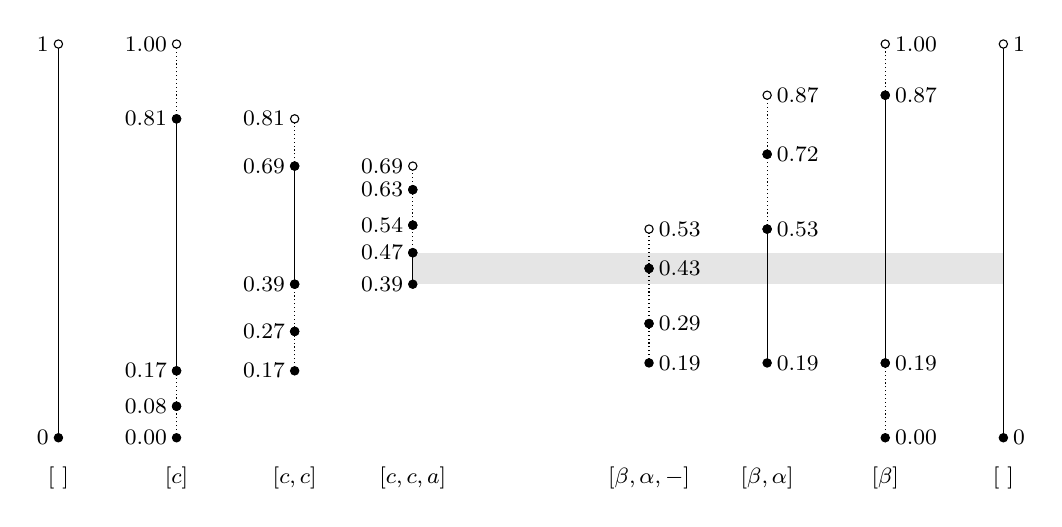
\begin{tikzpicture}[scale=0.05]
		% Final interval range
		\fill [opacity=0.1] (-30,0.39*100) rectangle (120,0.47*100);

		% Input side
		\intervalBothLabels{-120}{0}{100}{0}{1}{solid}{left}
		\node[below] at (-120,-5) {\footnotesize $[~]$};

		\intervalBothLabels{-90}{0}{100}{0.81}{1.00}{densely dotted}{left}
		\intervalBottomLabel{-90}{0}{100}{0.17}{0.81}{solid}{left}
		\intervalBottomLabel{-90}{0}{100}{0.08}{0.17}{densely dotted}{left}
		\intervalBottomLabel{-90}{0}{100}{0.00}{0.08}{densely dotted}{left}
		\node[below] at (-90,-5) {\footnotesize $[c]$};

		\intervalBothLabels{-60}{0}{100}{0.69}{0.81}{densely dotted}{left}
		\intervalBottomLabel{-60}{0}{100}{0.39}{0.69}{solid}{left}
		\intervalBottomLabel{-60}{0}{100}{0.27}{0.39}{densely dotted}{left}
		\intervalBottomLabel{-60}{0}{100}{0.17}{0.27}{densely dotted}{left}
		\node[below] at (-60,-5) {\footnotesize $[c,c]$};

		\intervalBottomLabel{-30}{0}{100}{0.39}{0.47}{solid}{left}
		\intervalBottomLabel{-30}{0}{100}{0.47}{0.54}{densely dotted}{left}
		\intervalBottomLabel{-30}{0}{100}{0.54}{0.63}{densely dotted}{left}
		\intervalBothLabels{-30}{0}{100}{0.63}{0.69}{densely dotted}{left}
		\node[below] at (-30,-5) {\footnotesize $[c,c,a]$};

		% Output side
		\intervalBothLabels{120}{0}{100}{0}{1}{solid}{right}
		\node[below] at (120,-5) {\footnotesize $[~]$};

		\intervalBothLabels{90}{0}{100}{0.87}{1.00}{densely dotted}{right}
		\intervalBottomLabel{90}{0}{100}{0.19}{0.87}{solid}{right}
		\intervalBottomLabel{90}{0}{100}{0.00}{0.19}{densely dotted}{right}
		\node[below] at (90,-5) {\footnotesize $[\beta]$};

		\intervalBothLabels{60}{0}{100}{0.72}{0.87}{densely dotted}{right}
		\intervalBottomLabel{60}{0}{100}{0.53}{0.72}{densely dotted}{right}
		\intervalBottomLabel{60}{0}{100}{0.19}{0.53}{solid}{right}
		\node[below] at (60,-5) {\footnotesize $[\beta,\alpha]$};

		\intervalBothLabels{30}{0}{100}{0.43}{0.53}{densely dotted}{right}
		\intervalBottomLabel{30}{0}{100}{0.29}{0.43}{densely dotted}{right}
		\intervalBottomLabel{30}{0}{100}{0.19}{0.29}{densely dotted}{right}
		\node[below] at (30,-5) {\footnotesize $[\beta,\alpha,-]$};

	\end{tikzpicture}

	\caption{\label{fig:interval_algorithm}Example run of the interval algorithm. The source emits symbols over the alphabet $\{a,b,c,d\}$, the target -- $\{\alpha,\beta,\gamma\}$. On the left, an input sequence $[c,c,a]$ from the source process gets mapped to $[0.39,0.47)$. On the right, this interval allows to generate up to 2 terms of an output sequence from the target process, \ie $[\beta,\alpha]$, which corresponds to $[0.19,0.53)$. Note that it is not possible to generate more terms of the output sequence, as neither $[0.19,0.29)$ nor $[0.29,0.43)$ nor $[0.43,0.53)$ is a superinterval of $[0.39,0.47)$.}

\end{figure}

I will denote by \intervalAlgorithm{I}{O} an instance of the interval algorithm configured for an input stochastic process $\mathcal I$ and an output stochastic process $\mathcal O$.

\subsection{Extension to multiple input processes}

It is possible to extend the interval algorithm to a scenario where the input sequence is a concatenation of sequences emitted by $N$ stochastic processes $\mathcal I_1, \dots, \mathcal I_N$. The input processes need to be defined over different alphabets $\mathfrak I_1, \dots, \mathfrak I_N$. We can see that this extension does not pose any problems as long as the alphabets are different. When mapping input sequence to an interval, it is clear which process a given term was emitted by, thus the appropriate conditional probability subintervals can be found. The rest of the algorithm proceeds as before. I will denote by $\angled{\mathcal I_1, \dots, \mathcal I_N / \mathcal O}$ an instance of the interval algorithm modified in such a way.

Note that if the processes are infinite, it is not possible to do the opposite, \ie define an interval algorithm $\angled{\mathcal I / \mathcal O_1, \dots, \mathcal O_N}$. It would end up being equivalent to simply $\angled{\mathcal I / \mathcal O_1}$.

\clearpage
\section{Stegosystem}
\label{sec:stegosystem}

In this section I will describe a simple stegosystem which allows to disguise an output sequence from one arbitrary stochastic process as a sequence which appears to have been generated by another arbitrary stochastic process. I will then describe how it is possible to construct a secure stegosystem with deniable encryption.

\FloatBarrier
\subsection{Simple stegosystem}
\label{sec:simple_stegosystem}

The interval algorithm described in \cref{sec:interval_algorithm} can be used to construct a simple stegosystem that generates \emph{stegotext} from \emph{plaintext}\footnote{Note that \emph{plaintext} has a very precise meaning in this context -- the unencrypted message. \emph{Plain text} written separately simply refers to an unformatted sequence of characters.}. Input plaintext sequence $\mathbf P$ on alphabet $\mathfrak P$ needs to have been generated according to a known stochastic process $\mathcal P$. An output stegotext sequence $\mathbf S$ on alphabet $\mathfrak S$ will be deterministically generated from $\mathbf P$ according to the statistics of an arbitrarily chosen stochastic process $\mathcal S$. Knowledge of $\mathbf S$ will allow to recover $\mathbf{P'}$ -- a sequence on $\mathfrak P$ whose prefix is $\mathbf P$.

For example, if we want to transmit information that is optimally compressed to binary, $\mathcal P$ will be \iid uniform. If we want the stegotext to be English text, we will use the English language model from \cref{sec:language_model} as $\mathcal S$.

Note that it is necessary to terminate $\mathbf P$ with an end-of-message symbol, or otherwise transmit its length, if we want to be able to uniquely recover $\mathbf P$ from $\mathbf{P'}$. This issue will be addressed later.

\subsubsection{Detailed description of the system}

The stegosystem requires a source of randomness $\mathcal R$ that outputs an infinite sequence $\mathbf R$ on alphabet $\mathfrak R$. $\mathcal R$ can be an arbitrary stochastic process with known statistics, for example a sequence of \iid uniform bits.

The sequence $\mathbf P$ is concatenated with $\mathbf R$ to create an infinite sequence $\mathbf I$. With \intervalAlgorithm{P,R}{S} we can use $\mathbf I$ to deterministically generate an arbitrarily long output sequence $\mathbf S$. It remains to show that a sufficiently long $\mathbf S$ allows us to find a correct sequence $\mathbf P'$. Remember that $\mathbf{P'}$ is defined as a sequence on $\mathfrak P$ whose prefix is $\mathbf P$.

To recover $\mathbf P$ from $\mathbf S$, we can run the interval algorithm \intervalAlgorithm{S}{P} with $\mathbf S$ as input. The only requirement to correctly decode all symbols of $\mathbf P$ is that $\mathbf s \subseteq \mathbf p$. This is the reason we used the process $\mathcal R$ during generation of $\mathbf S$ -- we kept refining the input interval $\mathbf i$ until it got small enough that $\mathbf s \subseteq \mathbf p$. $\mathbf s$ was guaranteed to decrease every time a new symbol is appended to $\mathbf S$ since the conditional probabilities are always less than 1.\footnote{Each symbol has a non-zero probability and the alphabet size of obviously more than 1.} \cref{fig:stegosystem_encoding} illustrates the procedure with a concrete example.

\begin{figure}[h!]
	\centering

	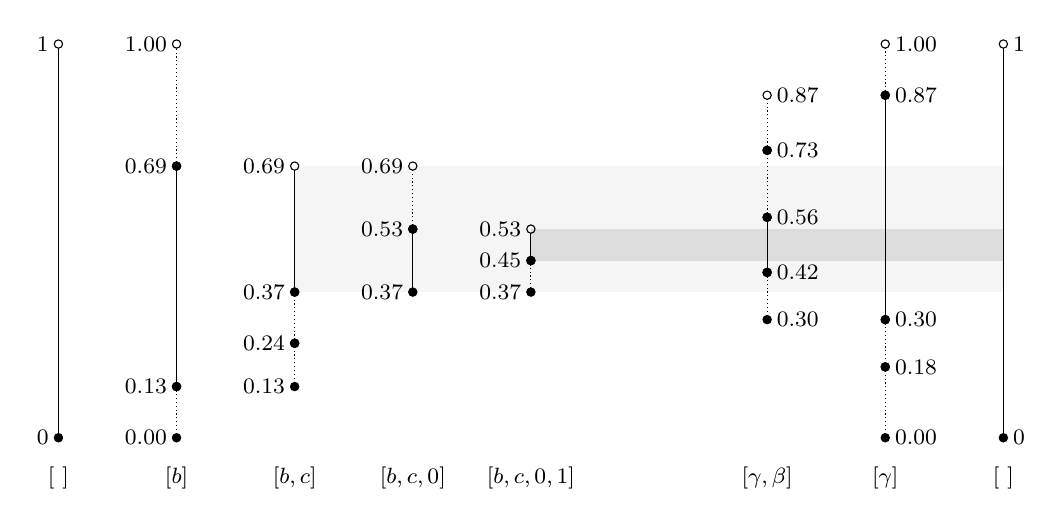
\begin{tikzpicture}[scale=0.05]
		% P interval range
		\fill [opacity=0.04] (-60,0.37*100) rectangle (120,0.69*100);
		
		% I interval range
		\fill [opacity=0.1] (0,0.45*100) rectangle (120,0.53*100);

		% Input side
		\intervalBothLabels{-120}{0}{100}{0}{1}{solid}{left}
		\node[below] at (-120,-5) {\footnotesize $[~]$};

		\intervalBothLabels{-90}{0}{100}{0.69}{1.00}{densely dotted}{left}
		\intervalBottomLabel{-90}{0}{100}{0.13}{0.69}{solid}{left}
		\intervalBottomLabel{-90}{0}{100}{0.00}{0.13}{densely dotted}{left}
		\node[below] at (-90,-5) {\footnotesize $[b]$};

		\intervalBothLabels{-60}{0}{100}{0.37}{0.69}{solid}{left}
		\intervalBottomLabel{-60}{0}{100}{0.24}{0.37}{densely dotted}{left}
		\intervalBottomLabel{-60}{0}{100}{0.13}{0.24}{densely dotted}{left}
		\node[below] at (-60,-5) {\footnotesize $[b,c]$};

		\intervalBothLabels{-30}{0}{100}{0.53}{0.69}{densely dotted}{left}
		\intervalBottomLabel{-30}{0}{100}{0.37}{0.53}{solid}{left}
		\node[below] at (-30,-5) {\footnotesize $[b,c,0]$};

		\intervalBothLabels{0}{0}{100}{0.45}{0.53}{solid}{left}
		\intervalBottomLabel{0}{0}{100}{0.37}{0.45}{densely dotted}{left}
		\node[below] at (0,-5) {\footnotesize $[b,c,0,1]$};

		% Output side
		\intervalBothLabels{120}{0}{100}{0}{1}{solid}{right}
		\node[below] at (120,-5) {\footnotesize $[~]$};

		\intervalBothLabels{90}{0}{100}{0.87}{1.00}{densely dotted}{right}
		\intervalBottomLabel{90}{0}{100}{0.30}{0.87}{solid}{right}
		\intervalBottomLabel{90}{0}{100}{0.18}{0.30}{densely dotted}{right}
		\intervalBottomLabel{90}{0}{100}{0.00}{0.18}{densely dotted}{right}
		\node[below] at (90,-5) {\footnotesize $[\gamma]$};

		\intervalBothLabels{60}{0}{100}{0.73}{0.87}{densely dotted}{right}
		\intervalBottomLabel{60}{0}{100}{0.56}{0.73}{densely dotted}{right}
		\intervalBottomLabel{60}{0}{100}{0.42}{0.56}{solid}{right}
		\intervalBottomLabel{60}{0}{100}{0.30}{0.42}{densely dotted}{right}
		\node[below] at (60,-5) {\footnotesize $[\gamma, \beta]$};

	\end{tikzpicture}

	\caption{\label{fig:stegosystem_encoding}Generating $\mathbf S$ (right) from $\mathbf P$ (left). Both $\mathcal P$ and $\mathcal S$ are arbitrary stochastic processes defined over the alphabets $\mathfrak P = \{a,b,c\}$ and $\mathfrak S = \{\alpha,\beta,\gamma,\delta\}$. $\mathcal R$ emits \iid uniform bits. Statistics of the corresponding processes are used to provide mappings between sequences and intervals. We are given $\mathbf P = [b,c]$ and we wish to generate $\mathbf S$ from it. $\mathbf P$ corresponds to the light grey region $\mathbf p = [0.37,0.69)$, which only allows to generate $\mathbf S$ up to $[\gamma]$. Since $[0.30,0.87) \nsubseteq [0.37,0.69)$, $[\gamma]$ is not enough to identify a sequence with prefix $\mathbf P$. However, if we use $\mathcal R$ to extend $\mathbf P$ to $\mathbf I = [b,c,0,1]$, we obtain the refined input interval $\mathbf i = [0.45, 0.53)$ shown in dark grey. $\mathbf i$ allows us to generate $\mathbf S = [\gamma,\beta]$ with the required property that $\mathbf s \subseteq \mathbf p$.}

\end{figure}

The problem is that we have no control over how small the interval $\mathbf s$ that satisfies $\mathbf s \subseteq \mathbf p$ gets. Since we do not know how long $\mathbf P$ is, we do not know when to stop generating symbols from $\mathcal P$. It may happen that even the largest of the intervals satisfying this condition will allow us to decode \emph{more} than just $\mathbf P$. This is why the sequence we decode is $\mathbf{P'}$, not $\mathbf P$. See \cref{fig:stegosystem_decoding} for an example of such a situation.

\begin{figure}[h!]
	\centering

	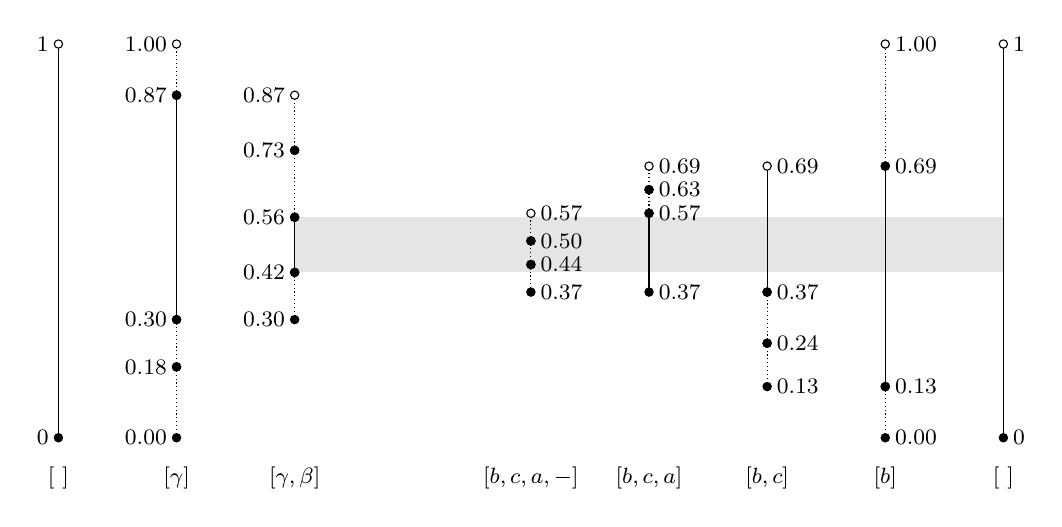
\begin{tikzpicture}[scale=0.05]
		% S interval range
		\fill [opacity=0.1] (-30,0.42*100) rectangle (150,0.56*100);

		% S side
		\intervalBothLabels{-90}{0}{100}{0}{1}{solid}{left}
		\node[below] at (-90,-5) {\footnotesize $[~]$};

		\intervalBothLabels{-60}{0}{100}{0.87}{1.00}{densely dotted}{left}
		\intervalBottomLabel{-60}{0}{100}{0.30}{0.87}{solid}{left}
		\intervalBottomLabel{-60}{0}{100}{0.18}{0.30}{densely dotted}{left}
		\intervalBottomLabel{-60}{0}{100}{0.00}{0.18}{densely dotted}{left}
		\node[below] at (-60,-5) {\footnotesize $[\gamma]$};

		\intervalBothLabels{-30}{0}{100}{0.73}{0.87}{densely dotted}{left}
		\intervalBottomLabel{-30}{0}{100}{0.56}{0.73}{densely dotted}{left}
		\intervalBottomLabel{-30}{0}{100}{0.42}{0.56}{solid}{left}
		\intervalBottomLabel{-30}{0}{100}{0.30}{0.42}{densely dotted}{left}
		\node[below] at (-30,-5) {\footnotesize $[\gamma, \beta]$};

		% P' side
		\intervalBothLabels{150}{0}{100}{0}{1}{solid}{right}
		\node[below] at (150,-5) {\footnotesize $[~]$};

		\intervalBothLabels{120}{0}{100}{0.69}{1.00}{densely dotted}{right}
		\intervalBottomLabel{120}{0}{100}{0.13}{0.69}{solid}{right}
		\intervalBottomLabel{120}{0}{100}{0.00}{0.13}{densely dotted}{right}
		\node[below] at (120,-5) {\footnotesize $[b]$};

		\intervalBothLabels{90}{0}{100}{0.37}{0.69}{solid}{right}
		\intervalBottomLabel{90}{0}{100}{0.24}{0.37}{densely dotted}{right}
		\intervalBottomLabel{90}{0}{100}{0.13}{0.24}{densely dotted}{right}
		\node[below] at (90,-5) {\footnotesize $[b,c]$};

		\intervalBothLabels{60}{0}{100}{0.63}{0.69}{densely dotted}{right}
		\intervalBottomLabel{60}{0}{100}{0.57}{0.63}{densely dotted}{right}
		\intervalBottomLabel{60}{0}{100}{0.37}{0.57}{solid}{right}
		\node[below] at (60,-5) {\footnotesize $[b,c,a]$};

		\intervalBothLabels{30}{0}{100}{0.50}{0.57}{densely dotted}{right}
		\intervalBottomLabel{30}{0}{100}{0.44}{0.50}{densely dotted}{right}
		\intervalBottomLabel{30}{0}{100}{0.37}{0.44}{densely dotted}{right}
		\node[below] at (30,-5) {\footnotesize $[b,c,a,-]$};

	\end{tikzpicture}

	\caption{\label{fig:stegosystem_decoding}Recovering $\mathbf{P'}$ (right) from $\mathbf S$ (left) using the interval algorithm \intervalAlgorithm{S}{P}. Since we don't know how long the original sequence $\mathbf P$ was, we keep generating terms according to the statistics of $\mathcal P$ for as long as possible. In this case we decode $\mathbf{P'} = [b,c,a]$. $\mathbf{P'}$ has the correct prefix $\mathbf P = [b,c]$, but also contains an extra symbol $a$.}

\end{figure}

\FloatBarrier
\subsection{Secure stegosystem}
\label{sec:secure_stegosystem}

The simple stegosystem from \cref{sec:simple_stegosystem} can be used to construct a secure stegosystem, where a key sequence $\mathbf K$ is used to \emph{securely} and \emph{innocuously} transform a plaintext sequence $\mathbf P$ to a stegotext sequence $\mathbf S$. Only the knowledge of $\mathbf K$ allows to recover from $\mathbf S$ a sequence with prefix $\mathbf P$.

\subsubsection{Generating secure stegotext}

The plaintext and key sequences are first mapped to intervals $\mathbf p$ and $\mathbf k$ in the usual way using their stochastic process models $\mathcal P$ and $\mathcal K$. They are then assigned binary sequences $\mathbf{P_2}$ and $\mathbf{K_2}$:

\begin{description}

\item[$\mathbf{P_2}$] \emph{Binary subinterval sequence} of $\mathbf p$, \ie the shortest sequence $\mathbf{P_2}$ such that $\mathbf {p_2} \subseteq \mathbf p$. Mapping between binary sequences and intervals is achieved in the usual way -- by successive refinements of the $[0,1)$ interval by its upper or lower half. Note that there may be more than one valid $\mathbf{P_2}$. See \cref{fig:plaintext_to_binary}.

\item[$\mathbf{K_2}$] \emph{Binary superinterval sequence} of $\mathbf k$, \ie the longest sequence $\mathbf{K_2}$ such that $\mathbf k \subseteq \mathbf {k_2}$. There is a single possible $\mathbf{K_2}$. Finding it is equivalent to generating $\mathbf{K_2}$ from $\mathbf K$ using the interval algorithm, so $\mathbf{K_2}$ is \iid uniform by construction. See \cref{fig:key_to_binary}.

\end{description}

The binary representation of plaintext $\mathbf{P_2}$ is then encrypted to binary \emph{ciphertext} $\mathbf{C_2}$ using a stream cipher with key $\mathbf{K_2}$. If $\mathbf{K_2}$ is at least as long as $\mathbf{P_2}$, we can achieve perfect secrecy \cite{shannon1949communication}. The simplest choice for a stream cipher is the \emph{exclusive or} operation between $\mathbf{P_2}$ and infinitely repeated key $\mathbf{K^+_2}$, \ie $\mathbf{C_2} = \mathbf{P_2} \oplus \mathbf{K^+_2}$.

$\mathbf{C_2}$ is used as an input to the simple stegosystem, producing pseudo-random English \emph{stegotext} $\mathbf S$. Note that $\mathbf{C_2}$ is used as $\mathbf P$ in \cref{sec:simple_stegosystem}. Provided that the language model is correct, the stegotext is statistically indistinguishable from any random English text.

\subsubsection{Recovering plaintext}

We can use the simple stegosystem to recover a binary sequence $\mathbf{C'_2}$ from $\mathbf S$. $\mathbf{C'_2}$ is a sequence whose prefix is $\mathbf{C_2}$, \ie the original input to the simple stegosystem. Knowing the key $\mathbf K$ and its binary representation $\mathbf{K_2}$, we can recover the original binary plaintext sequence potentially followed by more bits, \ie $\mathbf{P'_2} = \mathbf{C'_2} \oplus \mathbf{K^+_2}$.

$\mathbf {p'_2} \subseteq \mathbf {p_2} \subseteq \mathbf p$. The first relationship comes from the fact that $\mathbf{P_2}$ is a prefix of $\mathbf{P'_2}$ and the second holds because $\mathbf{P_2}$ is a binary subinterval sequence of $\mathbf p$. Using the language model we can now recover $\mathbf{P'}$, \ie the longest sequence such that $\mathbf {p'_2} \subseteq \mathbf {p'}$. $\mathbf{P'}$ will be the original plaintext $\mathbf P$ potentially followed by extra tokens.

\subsubsection{Deniable encryption}

An important feature of a stegosystem constructed in this way is \emph{deniable encryption}. Assume that an enemy with full knowledge of the system is told that a particular fragment of text $\mathbf S$ is indeed stegotext. Using the knowledge of the system (\ie the language model), they can reconstruct $\mathbf {C'_2}$ -- the binary ciphertext sequence with trailing bits.

However, the recovery of plaintext requires knowledge of the key. If a \emph{false key} $\mathbf {\overline K}$ is supplied in text form, it will still be correctly converted to its binary superinterval sequence $\mathbf {\overline K_2}$. It will then allow to decipher without failure ciphertext $\mathbf{C'_2}$ into an \emph{incorrect} binary sequence $\mathbf {\overline {P'}_2} = \mathbf{C'_2} \oplus \mathbf {\overline K^+_2}$. $\mathbf {\overline {P'}_2}$ will then be mapped to some incorrect plaintext $\mathbf {\overline {P'}}$, generated according to the stochastic process $\mathcal P$. So it will be a fragment of text randomly drawn from all English sentences.

A user asked to supply the key may give $\mathbf {\overline K}$ instead and claim that $\mathbf {\overline {P'}}$ contains the plaintext message as a prefix. If the enemy does not know $\mathbf P$ but expects it to be just a random sentence, \ie one generated according to the same statistics as $\mathcal P$, $\mathbf {\overline {P'}}$ is just as likely to contain $\mathbf P$ as a prefix as is the real $\mathbf{P'}$.

\subsubsection{Example}
\label{sec:secure_stegosystem_example}

Both plaintext and stegotext are generated according to the same stochastic process $\mathcal E$ over the alphabet of three tokens $\{ \alpha, \beta, \gamma \}$. The plaintext we wish to securely and innocuously transmit is $\mathbf P = [\beta,\gamma]$. For this purpose we use the key $\mathbf K = [\beta,\alpha]$.

\cref{fig:plaintext_to_binary,fig:key_to_binary,fig:ciphertext_to_stegotext} demonstrate generating the stegotext $\mathbf S = [\gamma,\alpha,\beta]$ from $\mathbf P$ and $\mathbf K$. \cref{fig:stegotext_to_ciphertext,fig:binary_to_plaintext} show recovering from the stegotext $\mathbf S$ a sequence $\mathbf{P'} = [\beta,\gamma,\beta]$ with prefix $\mathbf P$, given the knowledge of the key $\mathbf K$.

\begin{figure}[h]
	\centering

	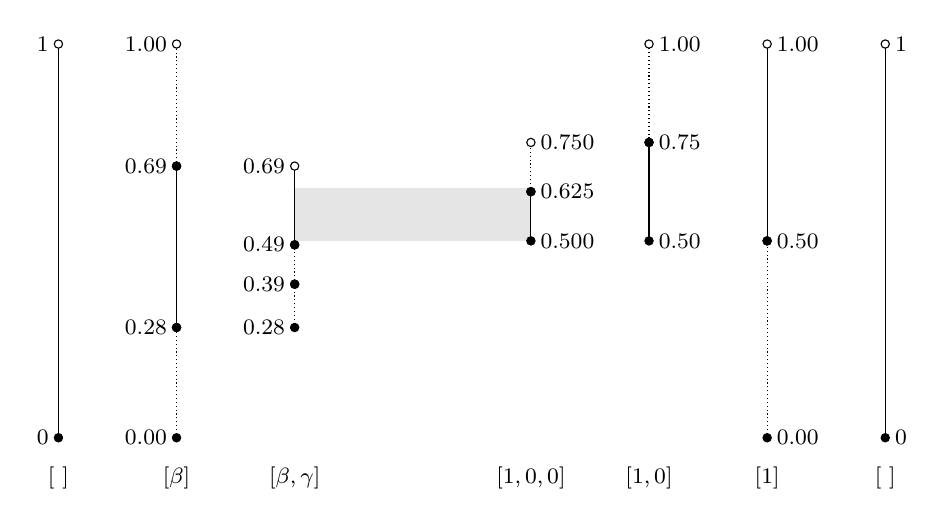
\begin{tikzpicture}[scale=0.05]
		% Show that the binary interval is a subinterval of plaintext interval
		\fill [opacity=0.1] (-30,0.500*100) rectangle (30,0.635*100);

		% Input side
		\intervalBothLabels{-90}{0}{100}{0}{1}{solid}{left}
		\node[below] at (-90,-5) {\footnotesize $[~]$};

		\intervalBothLabels{-60}{0}{100}{0.69}{1.00}{densely dotted}{left}
		\intervalBottomLabel{-60}{0}{100}{0.28}{0.69}{solid}{left}
		\intervalBottomLabel{-60}{0}{100}{0.00}{0.28}{densely dotted}{left}
		\node[below] at (-60,-5) {\footnotesize $[\beta]$};

		\intervalBothLabels{-30}{0}{100}{0.49}{0.69}{solid}{left}
		\intervalBottomLabel{-30}{0}{100}{0.39}{0.49}{densely dotted}{left}
		\intervalBottomLabel{-30}{0}{100}{0.28}{0.39}{densely dotted}{left}
		\node[below] at (-30,-5) {\footnotesize $[\beta,\gamma]$};

		% Output side
		\intervalBothLabels{120}{0}{100}{0}{1}{solid}{right}
		\node[below] at (120,-5) {\footnotesize $[~]$};

		\intervalBothLabels{90}{0}{100}{0.50}{1.00}{solid}{right}
		\intervalBottomLabel{90}{0}{100}{0.00}{0.50}{densely dotted}{right}
		\node[below] at (90,-5) {\footnotesize $[1]$};

		\intervalBothLabels{60}{0}{100}{0.75}{1.00}{densely dotted}{right}
		\intervalBottomLabel{60}{0}{100}{0.50}{0.75}{solid}{right}
		\node[below] at (60,-5) {\footnotesize $[1,0]$};

		\intervalBothLabels{30}{0}{100}{0.625}{0.750}{densely dotted}{right}
		\intervalBottomLabel{30}{0}{100}{0.500}{0.625}{solid}{right}
		\node[below] at (30,-5) {\footnotesize $[1,0,0]$};

	\end{tikzpicture}

	\caption{\label{fig:plaintext_to_binary}Converting the plaintext $\mathbf P = [\beta,\gamma]$ to a binary sequence $\mathbf{P_2} = [1,0,0]$. $\mathbf{P_2}$ is a binary subinterval sequence of the plaintext interval $\mathbf p = [0.49,0.69)$.}

\end{figure}

\begin{figure}[h]
	\centering

	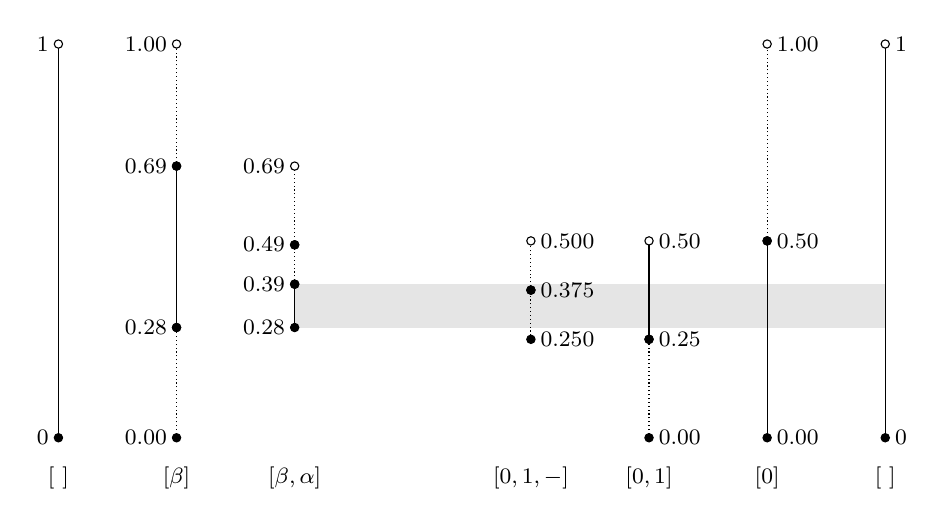
\begin{tikzpicture}[scale=0.05]
		% Show that the binary interval is a subinterval of plaintext interval
		\fill [opacity=0.1] (-30,0.28*100) rectangle (120,0.39*100);

		% Input side
		\intervalBothLabels{-90}{0}{100}{0}{1}{solid}{left}
		\node[below] at (-90,-5) {\footnotesize $[~]$};

		\intervalBothLabels{-60}{0}{100}{0.69}{1.00}{densely dotted}{left}
		\intervalBottomLabel{-60}{0}{100}{0.28}{0.69}{solid}{left}
		\intervalBottomLabel{-60}{0}{100}{0.00}{0.28}{densely dotted}{left}
		\node[below] at (-60,-5) {\footnotesize $[\beta]$};

		\intervalBothLabels{-30}{0}{100}{0.49}{0.69}{densely dotted}{left}
		\intervalBottomLabel{-30}{0}{100}{0.39}{0.49}{densely dotted}{left}
		\intervalBottomLabel{-30}{0}{100}{0.28}{0.39}{solid}{left}
		\node[below] at (-30,-5) {\footnotesize $[\beta,\alpha]$};

		% Output side
		\intervalBothLabels{120}{0}{100}{0}{1}{solid}{right}
		\node[below] at (120,-5) {\footnotesize $[~]$};

		\intervalBothLabels{90}{0}{100}{0.50}{1.00}{densely dotted}{right}
		\intervalBottomLabel{90}{0}{100}{0.00}{0.50}{solid}{right}
		\node[below] at (90,-5) {\footnotesize $[0]$};

		\intervalBothLabels{60}{0}{100}{0.25}{0.50}{solid}{right}
		\intervalBottomLabel{60}{0}{100}{0.00}{0.25}{densely dotted}{right}
		\node[below] at (60,-5) {\footnotesize $[0,1]$};

		\intervalBothLabels{30}{0}{100}{0.375}{0.500}{densely dotted}{right}
		\intervalBottomLabel{30}{0}{100}{0.250}{0.375}{densely dotted}{right}
		\node[below] at (30,-5) {\footnotesize $[0,1,-]$};

	\end{tikzpicture}

	\caption{\label{fig:key_to_binary}Converting the key $\mathbf K = [\beta,\alpha]$ to a binary sequence $\mathbf{K_2} = [0,1]$. $\mathbf{K_2}$ is the binary superinterval sequence of the key interval $\mathbf k = [0.28,0.39)$. We are effectively using the interval algorithm \intervalAlgorithm{E}{B}, where $\mathcal B$ denotes a source of \iid uniform bits.}

\end{figure}

\begin{figure}[h]
	\centering

	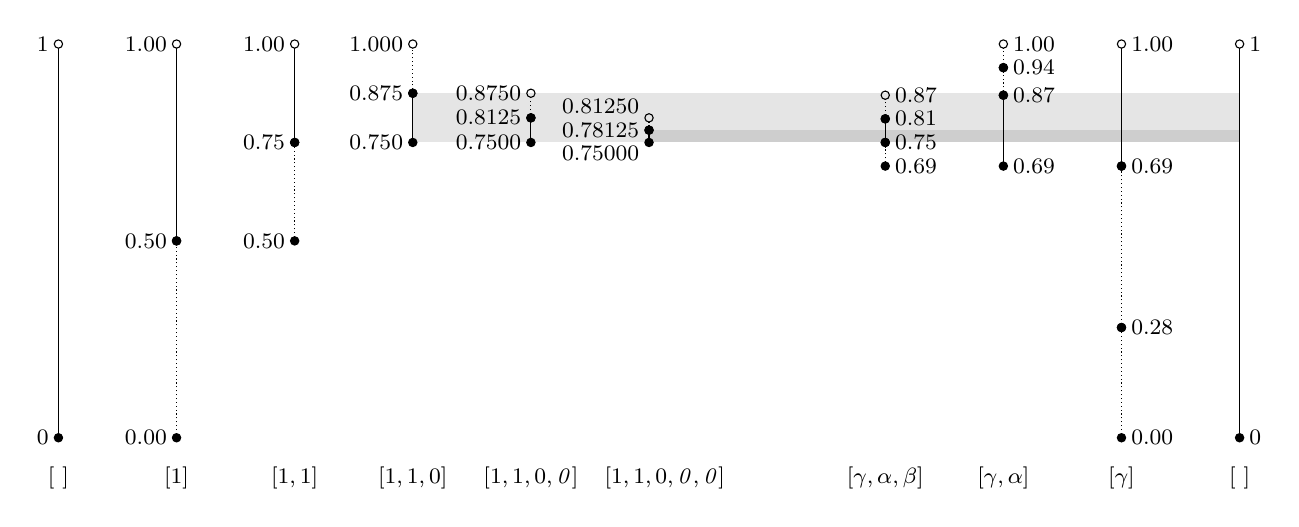
\begin{tikzpicture}[scale=0.05]
		% C_2 interval range
		\fill [opacity=0.1] (-90,0.750*100) rectangle (120,0.875*100);

		% I interval range
		\fill [opacity=0.1] (-30,0.7500*100) rectangle (120,0.78125*100);

		% C_2
		\intervalBothLabels{-180}{0}{100}{0}{1}{solid}{left}
		\node[below] at (-180,-5) {\footnotesize $[~]$};

		\intervalBothLabels{-150}{0}{100}{0.50}{1.00}{solid}{left}
		\intervalBottomLabel{-150}{0}{100}{0.00}{0.50}{densely dotted}{left}
		\node[below] at (-150,-5) {\footnotesize $[1]$};

		\intervalBothLabels{-120}{0}{100}{0.75}{1.00}{solid}{left}
		\intervalBottomLabel{-120}{0}{100}{0.50}{0.75}{densely dotted}{left}
		\node[below] at (-120,-5) {\footnotesize $[1,1]$};

		\intervalBothLabels{-90}{0}{100}{0.875}{1.000}{densely dotted}{left}
		\intervalBottomLabel{-90}{0}{100}{0.750}{0.875}{solid}{left}
		\node[below] at (-90,-5) {\footnotesize $[1,1,0]$};

		\intervalBothLabels{-60}{0}{100}{0.8125}{0.8750}{densely dotted}{left}
		\intervalBottomLabel{-60}{0}{100}{0.7500}{0.8125}{solid}{left}
		\node[below] at (-60,-5) {\footnotesize $[1,1,0,\mathit{0}]$};

		\interval{-30}{0}{100}{0.78125}{0.81250}{densely dotted}{left}
		\interval{-30}{0}{100}{0.75000}{0.78125}{solid}{left}
		% Interval descriptions
		\node[left] at (-30,0.78125*100+6) {\footnotesize 0.81250};
		\node[left] at (-30,0.78125*100) {\footnotesize 0.78125};
		\node[left] at (-30,0.78125*100-6) {\footnotesize 0.75000};
		\node[below] at (-30,-5) {\footnotesize ~~~ $[1,1,0,\mathit{0,0}]$};

		% S
		\intervalBothLabels{120}{0}{100}{0}{1}{solid}{right}
		\node[below] at (120,-5) {\footnotesize $[~]$};

		\intervalBothLabels{90}{0}{100}{0.69}{1.00}{solid}{right}
		\intervalBottomLabel{90}{0}{100}{0.28}{0.69}{densely dotted}{right}
		\intervalBottomLabel{90}{0}{100}{0.00}{0.28}{densely dotted}{right}
		\node[below] at (90,-5) {\footnotesize $[\gamma]$};

		\intervalBothLabels{60}{0}{100}{0.94}{1.00}{densely dotted}{right}
		\intervalBottomLabel{60}{0}{100}{0.87}{0.94}{densely dotted}{right}
		\intervalBottomLabel{60}{0}{100}{0.69}{0.87}{solid}{right}
		\node[below] at (60,-5) {\footnotesize $[\gamma,\alpha]$};

		\intervalBothLabels{30}{0}{100}{0.81}{0.87}{densely dotted}{right}
		\intervalBottomLabel{30}{0}{100}{0.75}{0.81}{solid}{right}
		\intervalBottomLabel{30}{0}{100}{0.69}{0.75}{densely dotted}{right}
		\node[below] at (30,-5) {\footnotesize $[\gamma,\alpha,\beta]$};

	\end{tikzpicture}

	\caption{\label{fig:ciphertext_to_stegotext}Generating stegotext $\mathbf S = [\gamma,\alpha,\beta]$ from ciphertext $\mathbf{C_2} = [1,1,0]$. Ciphertext is constructed by the \emph{exclusive or} operation on streams of $\mathbf{P_2}$ and the cycled key $\mathbf{K^+_2} = [0,1,0,1,0,1,\dots]$, \ie $\mathbf {C_2} = \mathbf{P_2} \oplus \mathbf{K^+_2} = [1,1,0]$. Ciphertext needs to be extended to $\mathbf I = [1,1,0,\mathit{0,0}]$ so that $\mathbf s \subseteq \mathbf{c_2}$, \ie $[0.75,0.81) \subseteq [0.750,0.875)$. Note that the stegotext is not unique -- if we extended the ciphertext to $\mathbf I = [1,1,0,\mathit{1,0}]$, the stegotext would be $\mathbf S = [\gamma,\alpha,\gamma]$.}

\end{figure}

\begin{figure}[h]
	\centering

	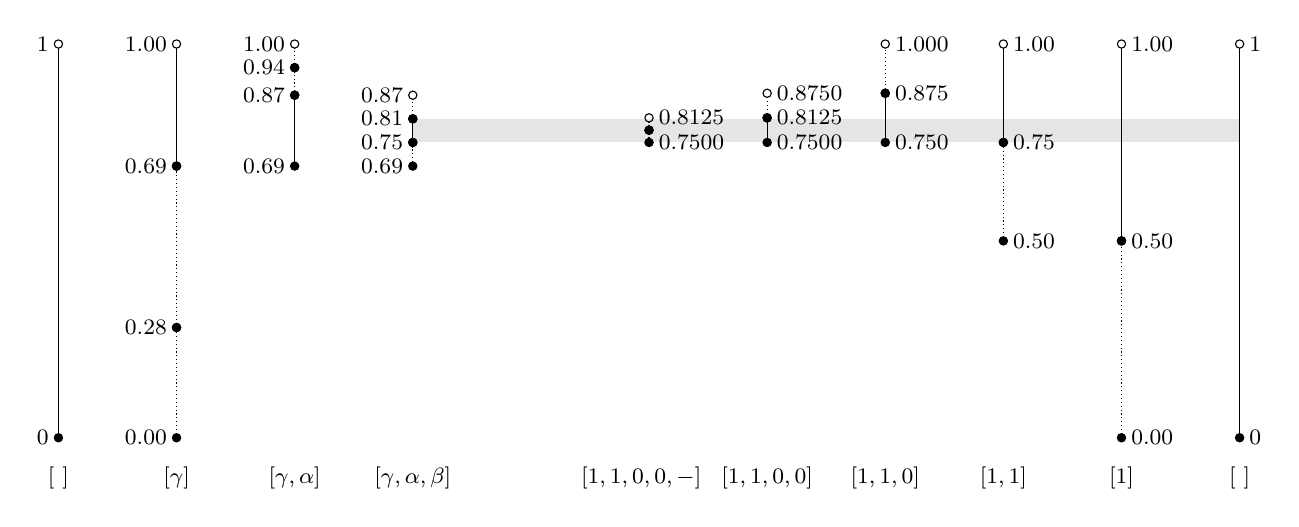
\begin{tikzpicture}[scale=0.05]
		% S interval range
		\fill [opacity=0.1] (-30,0.75*100) rectangle (180,0.81*100);

		% S
		\intervalBothLabels{-120}{0}{100}{0}{1}{solid}{left}
		\node[below] at (-120,-5) {\footnotesize $[~]$};

		\intervalBothLabels{-90}{0}{100}{0.69}{1.00}{solid}{left}
		\intervalBottomLabel{-90}{0}{100}{0.28}{0.69}{densely dotted}{left}
		\intervalBottomLabel{-90}{0}{100}{0.00}{0.28}{densely dotted}{left}
		\node[below] at (-90,-5) {\footnotesize $[\gamma]$};

		\intervalBothLabels{-60}{0}{100}{0.94}{1.00}{densely dotted}{left}
		\intervalBottomLabel{-60}{0}{100}{0.87}{0.94}{densely dotted}{left}
		\intervalBottomLabel{-60}{0}{100}{0.69}{0.87}{solid}{left}
		\node[below] at (-60,-5) {\footnotesize $[\gamma,\alpha]$};

		\intervalBothLabels{-30}{0}{100}{0.81}{0.87}{densely dotted}{left}
		\intervalBottomLabel{-30}{0}{100}{0.75}{0.81}{solid}{left}
		\intervalBottomLabel{-30}{0}{100}{0.69}{0.75}{densely dotted}{left}
		\node[below] at (-30,-5) {\footnotesize $[\gamma,\alpha,\beta]$};

		% C_2
		\intervalBothLabels{180}{0}{100}{0}{1}{solid}{right}
		\node[below] at (180,-5) {\footnotesize $[~]$};

		\intervalBothLabels{150}{0}{100}{0.50}{1.00}{solid}{right}
		\intervalBottomLabel{150}{0}{100}{0.00}{0.50}{densely dotted}{right}
		\node[below] at (150,-5) {\footnotesize $[1]$};

		\intervalBothLabels{120}{0}{100}{0.75}{1.00}{solid}{right}
		\intervalBottomLabel{120}{0}{100}{0.50}{0.75}{densely dotted}{right}
		\node[below] at (120,-5) {\footnotesize $[1,1]$};

		\intervalBothLabels{90}{0}{100}{0.875}{1.000}{densely dotted}{right}
		\intervalBottomLabel{90}{0}{100}{0.750}{0.875}{solid}{right}
		\node[below] at (90,-5) {\footnotesize $[1,1,0]$};

		\intervalBothLabels{60}{0}{100}{0.8125}{0.8750}{densely dotted}{right}
		\intervalBottomLabel{60}{0}{100}{0.7500}{0.8125}{solid}{right}
		\node[below] at (60,-5) {\footnotesize $[1,1,0,0]$};

		\intervalTopLabel{30}{0}{100}{0.78125}{0.8125}{densely dotted}{right}
		\intervalBottomLabel{30}{0}{100}{0.7500}{0.78125}{densely dotted}{right}
		\node[below] at (30,-5) {\footnotesize $[1,1,0,0,-]$~~~};

	\end{tikzpicture}

	\caption{\label{fig:stegotext_to_ciphertext}Recovering the ciphertext with trailing bits $\mathbf{C'_2} = [1,1,0,0]$ from the stegotext $\mathbf S = [\gamma,\alpha,\beta]$. We are effectively using the interval algorithm \intervalAlgorithm{E}{B}. Since the recipient of the message knows $\mathbf K$, $\mathbf {K_2} = [0,1]$ can be obtained exactly as in \cref{fig:key_to_binary}. Deciphered binary plaintext with trailing bits is then $\mathbf {P'_2} = \mathbf{C'_2} \oplus \mathbf {K^+_2} = [1,0,0,1]$. We can verify that $\mathbf {P'_2}$ has the prefix $\mathbf {P_2} = [1,0,0]$.}

\end{figure}

\begin{figure}[h]
	\centering

	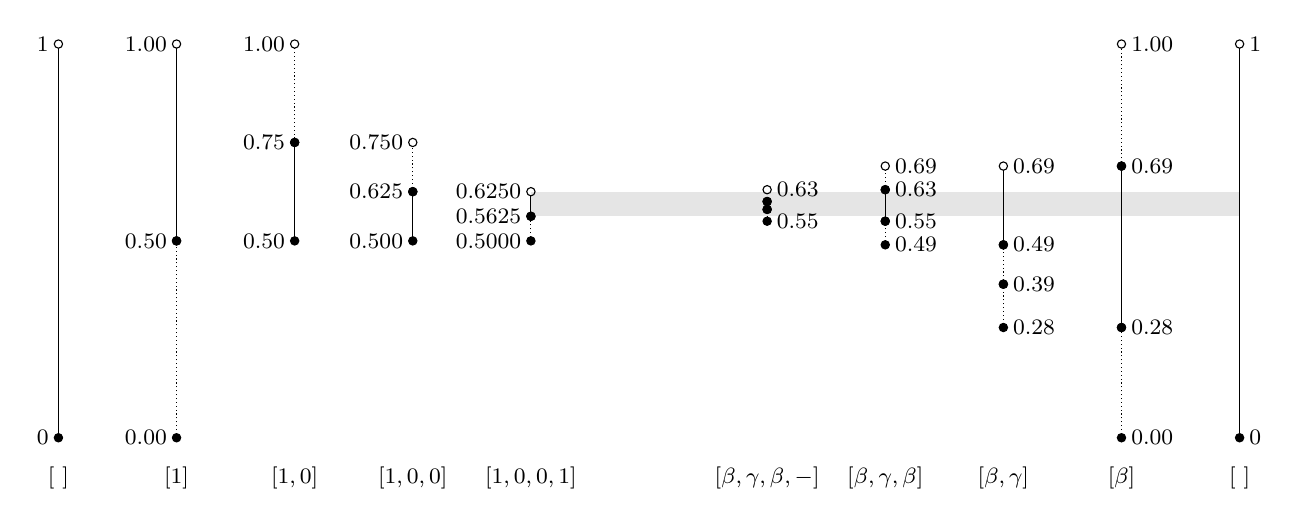
\begin{tikzpicture}[scale=0.05]
		% P'_2 interval
		\fill [opacity=0.1] (-30,0.5625*100) rectangle (150,0.6250*100);

		% P'_2
		\intervalBothLabels{-150}{0}{100}{0}{1}{solid}{left}
		\node[below] at (-150,-5) {\footnotesize $[~]$};

		\intervalBothLabels{-120}{0}{100}{0.50}{1.00}{solid}{left}
		\intervalBottomLabel{-120}{0}{100}{0.00}{0.50}{densely dotted}{left}
		\node[below] at (-120,-5) {\footnotesize $[1]$};

		\intervalBothLabels{-90}{0}{100}{0.75}{1.00}{densely dotted}{left}
		\intervalBottomLabel{-90}{0}{100}{0.50}{0.75}{solid}{left}
		\node[below] at (-90,-5) {\footnotesize $[1,0]$};

		\intervalBothLabels{-60}{0}{100}{0.625}{0.750}{densely dotted}{left}
		\intervalBottomLabel{-60}{0}{100}{0.500}{0.625}{solid}{left}
		\node[below] at (-60,-5) {\footnotesize $[1,0,0]$};

		\intervalBothLabels{-30}{0}{100}{0.5625}{0.6250}{solid}{left}
		\intervalBottomLabel{-30}{0}{100}{0.5000}{0.5625}{densely dotted}{left}
		\node[below] at (-30,-5) {\footnotesize $[1,0,0,1]$};

		% P'
		\intervalBothLabels{150}{0}{100}{0}{1}{solid}{right}
		\node[below] at (150,-5) {\footnotesize $[~]$};

		\intervalBothLabels{120}{0}{100}{0.69}{1.00}{densely dotted}{right}
		\intervalBottomLabel{120}{0}{100}{0.28}{0.69}{solid}{right}
		\intervalBottomLabel{120}{0}{100}{0.00}{0.28}{densely dotted}{right}
		\node[below] at (120,-5) {\footnotesize $[\beta]$};

		\intervalBothLabels{90}{0}{100}{0.49}{0.69}{solid}{right}
		\intervalBottomLabel{90}{0}{100}{0.39}{0.49}{densely dotted}{right}
		\intervalBottomLabel{90}{0}{100}{0.28}{0.39}{densely dotted}{right}
		\node[below] at (90,-5) {\footnotesize $[\beta,\gamma]$};

		\intervalBothLabels{60}{0}{100}{0.63}{0.69}{densely dotted}{right}
		\intervalBottomLabel{60}{0}{100}{0.55}{0.63}{solid}{right}
		\intervalBottomLabel{60}{0}{100}{0.49}{0.55}{densely dotted}{right}
		\node[below] at (60,-5) {\footnotesize $[\beta,\gamma,\beta]$};

		\intervalTopLabel{30}{0}{100}{0.60}{0.63}{densely dotted}{right}
		\interval{30}{0}{100}{0.58}{0.60}{solid}{right}
		\intervalBottomLabel{30}{0}{100}{0.55}{0.58}{densely dotted}{right}
		\node[below] at (30,-5) {\footnotesize $[\beta,\gamma,\beta,-]$};

	\end{tikzpicture}

	\caption{\label{fig:binary_to_plaintext}Recovering the plaintext with trailing symbols $\mathbf{P'} = [\beta,\gamma,\beta]$ from the binary plaintext with trailing bits $\mathbf{P'_2} = [1,0,0,1]$. $\mathbf {P'}$ has indeed the prefix $\mathbf P = [\beta,\gamma]$, so the stegosystem works correctly.}

\end{figure}

\clearpage
\section{Results}

In this section I will present the results of my project. I have implemented the full language model from \cref{sec:language_model} along with the secure stegosystem from \cref{sec:secure_stegosystem}.

\subsection{Generating random English sentences}

It is possible to use the language model from \cref{sec:language_model} and the interval algorithm from \cref{sec:interval_algorithm} to generate random English sentences. The procedure requires a sequence $\mathbf I$ emitted from a source of randomness -- an arbitrary stochastic process $\mathcal I$. $\mathbf I$ is then used as an input to an interval algorithm \intervalAlgorithm{I}{E}, where $\mathcal E$ denotes the stochastic process of English text.

I used \iid uniform bits generated by Python's \texttt{random.SystemRandom} class as $\mathcal I$. See \cref{sec:random_english_sentences} for examples of sentences generated in a 5-gram model using different combinations of parameters $\beta$, $\gamma$ and $F$.

\cref{tab:random_sentence_statistics} shows statistics of sample sentences generated using at least 2048 random bits (the output is continued until the end of the current sentence is reached). \emph{Perplexity per word} of a fragment of text consisting of $L$ tokens is defined in bits as $- \frac {1}{L} \log_2 P(w_1^L)$. It can be interpreted as the expected negative log probability of a token. Note that sample size is too small for the differences in \emph{average sentence length} to be statistically significant.

\begin{table}[h]
	\centering
	\begin{tabular}{ c | c | c || c | c}
	$\beta$ & $\gamma$ & $F$ & Perplexity per word & Av.\ sentence length \\
	\hline
	1 & 0.01 & 39 & 5.5 bits & 20 \\
	0.5 & 0.05 & 39 & 5.3 bits & 21 \\
	0.1 & 0.01 & 39 & 4.1 bits & 20 \\ \hline
	1 & 0.01 & 35 & 6.1 bits & 24 \\
	0.5 & 0.05 & 35 & 5.6 bits & 20 \\
	0.1 & 0.01 & 35 & 4.3 bits & 18 \\ \hline
	1 & 0.01 & 25 & 5.5 bits & 27 \\
	0.5 & 0.05 & 25 & 5.4 bits & 17 \\
	0.1 & 0.01 & 25 & 3.8 bits & 18 \\ \hline
	1 & 0.01 & 10 & 6.0 bits & 21 \\
	0.5 & 0.05 & 10 & 5.3 bits & 20 \\
	0.1 & 0.01 & 10 & 3.9 bits & 20 \\ \hline
	1 & 0.01 & 0 & 6.1 bits & 26 \\
	0.5 & 0.05 & 0 & 5.8 bits & 20 \\
	0.1 & 0.01 & 0 & 4.3 bits & 22
	\end{tabular}
	\caption{\label{tab:random_sentence_statistics}Statistics of random English sentences generated using the interval algorithm and the English language model with varying parameter values.}
\end{table}

\clearpage
\subsection{Secure stegosystem using the English language model}

I used the English language model for $N = 5$ and with parameters $\beta = 0.1$, $\gamma = 0.01$ and $F = 35$ to define a stochastic process $\mathcal E$. I then assumed that the plaintext, the key and the stegotext in the secure stegosystem from \cref{sec:secure_stegosystem} all have the statistics of $\mathcal E$.

\cref{tab:results_plaintext,tab:results_real_key,tab:results_false_key,tab:results_stegotext} demonstrate generating example stegotext and \cref{tab:results_correct_recovered_plaintext,tab:results_false_recovered_plaintext} recovering the plaintext using correct and incorrect keys. The procedure and notation are exactly the same as in the example from \cref{sec:secure_stegosystem_example}, so refer to it for a more detailed explanation of the method.

% Stretch arrays vertically
\renewcommand{\arraystretch}{1.25}

\begin{table}[h]
	\centering
	\begin{tabular}{m{3cm} m{12cm}}
	\centering plaintext & Come in the morning with the documents. \\ \hline
	\centering $\mathbf P$ & \_START\_ come in the morning with the documents .\ \_END\_ \\ \hline
	\centering $-\log_2 P(\mathbf P)$ & 53.9 bits \\ \hline
	\centering $\mathbf{P_2}$ & \footnotesize \texttt{0 1 0 0 0 0 1 0 1 1 0 1 1 0 1 0 0 0 0 1 1 1 0 1 0 0 0 1 1 1 0 0 1 0 0 1 1 1 1 0 0 0 0 0 0 1 0 0 1 1 1 0 1 0 0} \\ \hline
	\centering $| \mathbf{P_2} |$ & 55 bits
	\end{tabular}
	\caption{\label{tab:results_plaintext}Parsing plaintext $\mathbf P$ into a sequence of tokens and converting it to binary. Note that the sequence $\mathbf{P_2}$ contains $55 - 53.9 = 1.1~\text{bits}$ of redundant information content \wrt $\mathbf P$. This is because $\mathbf{P_2}$ needs to be a binary \emph{subinterval} sequence of $\mathbf P$. The difference is however never larger than 2 bits -- it is a known result from arithmetic coding.}
\end{table}

\begin{table}[h]
	\centering
	\begin{tabular}{m{3cm} m{12cm}}
	\centering real key & Light rain on Monday morning. \\ \hline
	\centering $\mathbf K$ & \_START\_ light rain on monday morning .\ \_END\_ \\ \hline
	\centering $-\log_2 P(\mathbf K)$ & 47.0 bits \\ \hline
	\centering $\mathbf{K_2}$ & \footnotesize \texttt{1 0 0 0 1 0 1 1 0 0 1 1 1 0 0 1 0 1 1 0 1 0 1 0 0 0 0 1 0 0 0 0 0 0 0 1 1 1 1 1 1 0 1 1 0 0} \\ \hline
	\centering $| \mathbf{K_2} |$ & 46 bits
	\end{tabular}
	\caption{\label{tab:results_real_key}Parsing the real key into a sequence of tokens and then converting it to binary. This time, $\mathbf{K_2}$ has fewer bits than $\mathbf K$ because it needs to be a binary \emph{superinterval} sequence. In other words, we cannot use all the information from $\mathbf K$ to generate $\mathbf{K_2}$.}
\end{table}

\begin{table}[h]
	\centering
	\begin{tabular}{m{3cm} m{12cm}}
	\centering false key & Early light rain or drizzle will soon die out. \\ \hline
	\centering $\mathbf{\overline K}$ & \_START\_ early light rain or drizzle will soon die out .\ \_END\_ \\ \hline
	\centering $-\log_2 P(\mathbf{\overline K})$ & 84.1 bits \\ \hline
	\centering $\mathbf {\overline K_2}$ & \footnotesize \texttt{0 1 0 0 1 1 0 0 0 0 0 1 1 1 0 1 0 0 1 0 0 1 0 0 1 0 0 1 1 1 0 1 0 0 1 1 0 1 0 0 0 1 0 1 1 0 1 0 0 0 1 1 1 0 0 0 1 0 0 1 0 1 0 0 0 1 1 1 0 1 0 1 0 1 0 1 0 1 1 0 1 0 1} \\ \hline
	\centering $|\mathbf {\overline K_2}|$ & 83 bits
	\end{tabular}
	\caption{\label{tab:results_false_key}Processing the false key in the same way as in \cref{tab:results_real_key}.}
\end{table}

\begin{table}[h]
	\centering
	\begin{tabular}{m{3cm} m{12cm}}
	\centering $\mathbf{C_2} = \mathbf{P_2} \oplus \mathbf{K^+_2}$ & \footnotesize \texttt{1 1 0 0 1 0 0 1 1 1 1 0 0 0 1 1 0 1 1 1 0 1 1 1 0 0 0 0 1 1 0 0 1 0 0 0 0 0 0 1 1 0 1 1 0 1 1 0 1 1 0 0 0 1 0} \\ \hline
	\centering $| \mathbf{C_2} |$ & 55 bits \\ \hline
	\centering $\mathbf S$ & \_START\_ the hurrian pantheon of the gods , o king , who is in turn responsible for the conditions at the surface of the whole earth , we could not talk to her about what she had done .\ \_END\_ \\ \hline
	\centering $-\log_2 P(\mathbf S)$ & 152.7 bits \\ \hline
	\centering stegotext & The Hurrian pantheon of the gods, o king, who is in turn responsible for the conditions at the surface of the whole Earth, we could not talk to her about what she had done. \\ \hline
	\centering $\mathbf{C'_2}$ & \footnotesize \texttt{1 1 0 0 1 0 0 1 1 1 1 0 0 0 1 1 0 1 1 1 0 1 1 1 0 0 0 0 1 1 0 0 1 0 0 0 0 0 0 1 1 0 1 1 0 1 1 0 1 1 0 0 0 1 0 1 0 0 0 1 1 1 0 1 0 1 1 0 1 0 1 0 0 1 0 0 1 1 0 1 1 1 0 0 0 1 1 0 1 1 1 0 0 0 0 1 1 0 1 0 0 1 0 0 0 0 0 1 1 1 1 0 0 1 1 1 1 0 0 1 1 1 0 0 0 0 1 0 0 1 1 1 1 0 0 1 1 0 1 1 0 1 0 0 1 1 0 1 0} \\ \hline
	\centering $| \mathbf{C'_2} |$ & 149 bits
	\end{tabular}
	\caption{\label{tab:results_stegotext}Generating stegotext using the real key. Note that the final stegotext has been formatted \emph{by hand} to appear more natural. Any modifications are allowed as long as the formatted text parses to the same sequence of tokens $\mathbf S$. The stegotext is very long -- its information content is almost 3 times that of the ciphertext $\mathbf{C_2}$, which it needs to identify. In total it contains $152.7 - 55 = 97.7~\text{bits}$ of redundant information. The large difference results from the fact that, in order to appear natural, the stegotext sequence needs to terminate at an \ngram{\_END\_} token. Since beyond the input sequence $\mathbf{C_2}$ the stegotext is generated truly randomly, in a different realisation the stegotext $\mathbf S$ could be shorter or even longer.}
\end{table}

\begin{table}[h]
	\centering
	\begin{tabular}{m{3cm} m{12cm}}
	\centering $\mathbf{P'_2} = \mathbf{C'_2} \oplus \mathbf{K^+_2}$ & \footnotesize \texttt{0 1 0 0 0 0 1 0 1 1 0 1 1 0 1 0 0 0 0 1 1 1 0 1 0 0 0 1 1 1 0 0 1 0 0 1 1 1 1 0 0 0 0 0 0 1 0 0 1 1 1 0 1 0 0 1 1 1 1 1 1 0 0 0 1 1 0 0 0 0 1 0 0 0 0 0 1 1 0 1 1 0 1 1 1 0 0 0 0 0 1 0 1 0 0 1 0 0 0 1 0 1 1 1 1 0 0 0 1 0 0 0 1 1 0 1 1 0 0 0 1 1 0 0 0 0 1 1 1 0 0 0 0 0 1 0 1 0 0 1 0 1 1 0 0 0 0 1 1} \\ \hline
	\centering $| \mathbf{P'_2} |$ & 149 bits \\ \hline
	\centering $\mathbf{P'}$ & \_START\_ come in the morning with the documents .\ \_END\_ \_START\_ the grocer takes the form of a human , or a full - time basis .\ \_END\_ \_START\_ with this \\ \hline
	\centering $-\log_2 P(\mathbf{P'})$ & 139.0 bits \\ \hline
	\centering recovered plaintext & Come in the morning with the documents.\ \ \emph{The grocer takes the form of a human, or a full-time basis.\ \ With this}
	\end{tabular}
	\caption{\label{tab:results_correct_recovered_plaintext}Recovering plaintext using the correct key. Note how the recovered sequence does \emph{not} have to terminate with an \ngram{\_END\_} token.}
\end{table}

\begin{table}[h]
	\centering
	\begin{tabular}{m{3cm} m{12cm}}
	\centering $\mathbf{\overline{P'}_2} = \mathbf{C'_2} \oplus \mathbf{\overline K^+_2}$ & \footnotesize \texttt{1 0 0 0 0 1 0 1 1 1 1 1 1 1 1 0 0 1 0 1 0 0 1 1 1 0 0 1 0 0 0 1 1 0 1 1 0 1 0 1 1 1 1 0 1 1 0 0 1 1 1 1 1 1 0 1 1 0 0 0 1 0 0 1 0 0 0 1 1 1 1 1 0 0 0 1 1 0 1 1 0 1 1 0 1 1 1 1 0 1 1 0 0 0 1 0 0 0 0 0 0 0 0 0 1 0 0 0 1 1 0 1 1 1 0 1 1 1 1 1 0 1 0 0 1 0 0 1 0 0 1 1 1 1 1 0 1 0 1 0 0 1 1 0 0 1 0 1 1} \\ \hline
	\centering $| \mathbf{\overline{P'}_2} |$ & 149 bits \\ \hline
	\centering $\mathbf{\overline{P'}}$ & \_START\_ jennings , h .\ s .\ ( editor ) .\ \_END\_ \_START\_ an abstruse and learned specialist who finds that he has been to the west of the entrance to the vagina .\ \_END\_ \_START\_ there is a suggestion that the earth might be blessed .\ \_END\_ \_START\_ \\ \hline
	\centering $-\log_2 P(\mathbf{\overline{P'}})$ & 145.8 bits \\ \hline
	\centering recovered false plaintext & Jennings, H.\ S.\ (editor).\ \ An abstruse and learned specialist who finds that he has been to the west of the entrance to the vagina.\ \ There is a suggestion that the Earth might be blessed.
	\end{tabular}
	\caption{\label{tab:results_false_recovered_plaintext}Recovering plaintext using an incorrect key.}
\end{table}

% Go back to normal array row size
\renewcommand{\arraystretch}{1}

\clearpage
\section{Discussion}

\subsection{Language model statistics and the rate of the stegosystem}

\subsubsection{Perplexity of a language model}

Perplexity per token in bits is the expected negative log probability of a token given the preceding ones. In the interval algorithm, it directly corresponds to the expected size of successive subintervals. It can be also interpreted as the number of bits of information needed on average to encode a single token. See \cite{brown1992entropy} for a broader treatment of perplexity in computational linguistics.

We can talk about perplexity of a probability distribution itself (first sense) and the perplexity of a probability distribution that tries to model some test data (second sense). The former applies to the generation of random sentences and describes the variety of text that can be produced by the model. For example, for a model with perplexity of 5.4 bits, generating the next token can be thought of as equivalent to choosing 1 out of $2^{5.4} \approx 42$ equally likely choices.

It can be trivially shown that an \iid uniform model has the highest possible perplexity. However, it is obviously not a good model of English. This is why language models are judged by the former criterion -- perplexity when modelling test data. It is directly related to the cross-entropy between the probability distribution of the model and the true probability distribution of test text. The lower the perplexity, the better the model predicts the next token.

\subsubsection{Plaintext model perplexity}

In the context of this project, when encoding the plaintext we should \emph{minimise} the perplexity in the second sense. We want the information to be optimally compressed. This can be achieved by learning and matching the probability distribution of plaintext. Indeed, this is how the interval algorithm works -- by mapping a sequence using its \emph{true} distribution.

\subsubsection{Stegotext model perplexity}

To maximise the rate of the system, the stegotext should be generated using a source with \emph{maximum} perplexity in the first sense. We want each output token to contain as much information as possible -- this is how we ensure that the information from plaintext is transmitted using as few stegotext tokens as possible. For example, if we only used the works of Shakespeare to model stegotext, there would not be much variety in the output sentences. As a result, we would need to output relatively long paragraphs of text. Conversely, if the sentences came from general English, each one would be relatively unlikely, so would contain a lot of information.

However, to ensure innocuousness, stegotext needs to be generated according to the same process as the text it aims to mimic. So we are again forced to match the stochastic process to fit particular training data.

\subsubsection{Rate of the stegosystem}

Knowing the perplexities of the plaintext and stegotext models, we can talk about the expected rate of the system, \ie the number of plaintext tokens that are on average transmitted using stegotext tokens. \cite{hanhoshi1997} gives lower and upper bounds for the expected length of the input sequence when generating a \emph{single} term from a discrete output probability distribution using the interval algorithm. The only property of the discrete output distribution it depends on is the entropy.

In principle, it should be possible to adapt this bound to the case of the stegosystem. Input and output should be simply reversed -- in the stegosystem it is the output that has to uniquely identify the input. We should also interpret plaintext as a discrete probability distribution over the set of \emph{all} possible plaintext sequences of length $L$. In this way, we will be able to talk about the entropy of plaintext as a function of $L$, the number of tokens we want to transmit.

There are two problems. Firstly, because of the prohibitive size of the dynamically generated conditional probability trees, none of the statistics of the two distributions can be calculated exactly -- we need to estimate them and motivate why the estimations are justified.

Secondly, in a practical stegosystem it is advantageous to continue generating stegotext randomly until the end of a sentence is reached. As a result, the stegotext does not awkwardly terminate mid-sentence. This lowers the rate, as some number of trailing tokens needs to be appended. It is not trivial to introduce this constraint when calculating bounds on the expected number of tokens of stegotext.

However, there is a number of \emph{common sense} relationships between model statistics and the rate, which I will state without proof:

\begin{enumerate}
\item The rate falls with plaintext perplexity.
\item The rate increases with stegotext perplexity.
\item The rate falls with average stegotext sentence length.
\end{enumerate}

\subsection{Unique recovery of plaintext}

\subsubsection{Communicating the length of plaintext}

The stegosystem as described in \cref{sec:simple_stegosystem} does not allow to uniquely identify plaintext from stegotext. We can only recover a sequence of tokens whose \emph{prefix} is the plaintext. If we want to know plaintext exactly, its length needs to be somehow communicated:

\begin{description}
	\item[EOM token] We can add an \emph{end of message} token to our alphabet. The problem is learning its conditional probabilities. We could constraint \ngram{\_EOM\_} to only follow an \ngram{\_END\_} token and then create a probability distribution over the number of sentences in the plaintext. We can choose for example a \pmf from the exponential family. The subinterval size corresponding to \ngram{\_EOM\_} would be then equal to the probability that the current sentence is the last one.
	\item[Communicating $L$ at the beginning of plaintext] We can transmit the length $L$ of plaintext as the first symbol. $[0,1)$ can be partitioned into an infinite number of arbitrarily sized intervals, each corresponding to a particular $L$. Thus, if we can measure the \pmf of $L$, we can exactly match it. If in practice we do not care about being optimal, we can use a binary integer prefix code to initially partition $[0,1)$ by lengths. The requirement is that every possible sequence of bits either is a codeword, is a prefix of a codeword, or has a codeword as a prefix -- then $[0,1)$ will be partitioned among all integers.
\end{description}

\subsubsection{Compromising innocuousness}

In the case of a simple stegosystem from \cref{sec:simple_stegosystem}, communicating the length of plaintext may compromise innocuousness. Real stegotext is guaranteed to have \emph{consistent plaintext length} -- we should either eventually decode an \ngram{\_EOM\_} token, or we should not decode more tokens than the number given by the length declaration.

This is not the case with truly random sentences interpreted as stegotext. If our stegosystem uses the \ngram{\_EOM\_} token, it is not guaranteed to appear within the recovered plaintext sequence. Similarly, if the plaintext length declaration gives $L$, we may in fact recover a plaintext sequence shorter than $L$.

As a result, plaintext length consistency increases the probability that observed fragment of text is stegotext. It is possible that length consistency is an \emph{almost sure} indication of using the stegosystem -- simulations or theoretical analysis should answer this question.

\subsubsection{Compromising security}

If we use the secure stegosystem from \cref{sec:secure_stegosystem}, innocuousness of transmission is not compromised in an obvious way. We cannot attempt to decode plaintext without knowing the key, so we do not know if its length will be consistent or not.

However, an enemy with partial knowledge can infer more information. For example, if the enemy knows that a fragment of text is stegotext, they also know that a key that gives inconsistent plaintext length is not correct -- deniable encryption no longer applies. If they know the key, the situation is completely analogous to the one in the previous section -- they have an above chance probability of guessing whether a given fragment of text is stegotext or not.

\subsection{Sentence delimiters}

Google Books $N$-grams contain \ngram{\_START\_} and \ngram{\_END\_} tokens to identify beginning and end of a sentence. If stegotext is \emph{generated} using the language model, it will inevitably contain these tokens. For example any sequence of full sentences will start with \ngram{\_START\_} and finish with \ngram{\_END\_}.

Some kind of convention needs to be adopted to uniquely identify sentence delimiters in \emph{formatted} output text. I decided to denote them by multiple whitespace characters, for example a double space. To avoid ambiguity, the empty sentence \ngram{\_START\_ \_END\_} is not allowed in the model.

This has non-trivial consequences for practical application of the system. Since real text rarely has such specific and explicit sentence boundaries, their presence is suspicious. In hindsight, choosing a corpus without explicit sentence start and end tokens would simplify matters. In addition, it would introduce desirable continuity between sentences.

Examples of corpora meeting this condition are the 2009 Google Books $N$-grams Corpus and the COCA $N$-grams discussed below.

\subsection{Using COCA instead of Google Books}

Sentences shown in \cref{sec:random_english_sentences} do not always look natural. They still contain some \emph{noise} (\ie rather meaningless punctuation characters and single letters placed next to each other), or even foreign words.

The first problem is partly amplified by normalising and exploding tokens, as described in \cref{sec:normalising_tokens,sec:exploding_tokens}. \cref{tab:normalisation_examples} in the first section shows that special characters are transliterated into basic punctuation, which is then exploded into multiple tokens. This is necessary to unambiguously interpret formatted text, but inflates the punctuation counts.

The aim of the Google Books project is to digitise \emph{all} books in the world. The corresponding $N$-gram corpus is only a side project, so source texts are not curated in any major way. On the other hand, the Corpus of Contemporary American English has been constructed specifically to be a large and balanced corpus suitable for linguistic analysis \cite{coca2010}.

I expect the COCA $N$-grams corpus to contain fewer special special characters or foreign words. Additionally, it does not have a cutoff on counts, which gives more flexibility in designing the language model. Its drawbacks compared to the Google Books $N$-grams are: price and counts given only up to $N=4$. It is not possible to be sure without implementing the COCA corpus, but I now expect it to be give better results in a practical system.

\clearpage
\section{Conclusions}

What I have done:

\begin{enumerate}
	\item Designed methods for processing $N$-grams corpora, among them:
	\item Designed a method for breaking complex, potentially overlapping $N$-grams into simpler ones and an algorithm for inducing the counts of simple $N$-grams from the complex ones
	\item Designed a format for storing $N$-grams corpora in a space-efficient way and $log(\text{size})$ access time
	\item Designed a language model which assign non-zero probability to every fragment of text
	\item Designed a method for estimating the amount of probability mass assigned to lower-order token conditional probability estimates
	\item Designed using the interval algorithm a simple stegosystem that masks the output of one arbitrary, discrete stochastic process as if it was the output of a different arbitrary process
	\item Designed a secure stegosystem that protects the output of the original process using a symmetric key and provides deniable encryption, \ie gives a plausible answer when decrypting the message using any incorrect key
	\item Implemented all of the above for the Google Books $N$-grams Corpus
\end{enumerate}

\clearpage
\footnotesize
\bibliographystyle{unsrt}
\bibliography{../bibliography}

\clearpage
\appendix
\section{Random English sentences}
\label{sec:random_english_sentences}

% 	tokenStrings: print token strings in fixed with font
%
%	#1	- escaped token strings
\newcommand{\tokenStrings}[1] {
	\footnotesize
	\begin{sloppypar}
	\texttt{#1}
	\end{sloppypar}
	\normalsize
}

\subsection{$N = 5$, $\beta = 1$, $\gamma = 0.01$, $F = 39$}

\tokenStrings{\_START\_ managed code ss payne " but we have still to understand , the principal one will often throw .\ \_END\_ \_START\_ the answer is clearly yes .\ \_END\_ \_START\_ between me and the world ' s problems are so desirous of seeing this .\ \_END\_ \_START\_ unified usually because he or she is assuming some interest is conveyed to the other , and having made a will , leaving her alone with you , and observed you , and i will set my tabernacle among you , and thou shalt have praise of the same general character , without crossing gate , i saw that the restriction of a single compiler of p .\ birthing : k .\ j .\ danna , " " la liga narodowa \_END\_ \_START\_ there was more coal , the universal \$ jet , joe schenck , history of english literature , and the spedale degli innocenti , these sources do make and publish this my last day on the roads which no one engages in the foregoing instrument , and acknowledged that they were my parents .\ " \_END\_ \_START\_ the military officers of the colony , " he said , " love is a nonprofit needs just a few hours earlier than had been expected ; \_END\_}

\subsection{$N = 5$, $\beta = 0.5$, $\gamma = 0.05$, $F = 39$}

\tokenStrings{\_START\_ but , two days later , and " be sure to come .\ " \_END\_ \_START\_ a lean black cat , with a > b , then the other conspirators and marcus brutus stab caesar too ? " \_END\_ \_START\_ in many instances the old flame of passion , and then the farm operator was a bare light bulb hanging from the ceiling .\ \_END\_ \_START\_ a year after this , before it was born , it seems to me only a month when he was in new york on his own .\ " \_END\_ \_START\_ chemical and microbiological properties of interest are the most important aspects of their preparation , and their lives were in jeopardy , and his mind was not made up by the use of effective contraception .\ \_END\_ \_START\_ anonymous .\ \_END\_ \_START\_ any outcome of the disease ( figure energy resources .\ \_END\_ \_START\_ even more important , such as : god , nature , and the philosophy of science : an introduction .\ " ) \_END\_ \_START\_ the size of all the particles of the solid phase .\ \_END\_ \_START\_ this has been especially true in the past and do not want a doctor , " she said .\ \_END\_}

\subsection{$N = 5$, $\beta = 0.1$, $\gamma = 0.01$, $F = 39$}

\tokenStrings{\_START\_ if a approachable because even after probable cause has been established .\ \_END\_ \_START\_ a day later , there was another one , usually by the chief resident , and all these things are after - effects of , randy ticks working analogous to our infant church , and that he was " a big guy like me er the deep their shadows fling , yon turret stands ; \_END\_ \_START\_ but should one not bringing the liquid is then passed on to the next and the next generation ' s concerto , " and in one of his books as well as a shrewd , but it ' s entirety , and also changes color within the meaning of ss existence to a higher sovereign than the commonwealth , for the purpose of tracing paper on which a king and queen , and who had so much to do with this ! \_END\_ \_START\_ ivanych .\ \_END\_ \_START\_ kangaroos successful in receiving the word of god and the immortality of the soul , strong in its natural state .\ \_END\_ \_START\_ fifteen minutes all night .\ \_END\_ \_START\_ the total number of optional " .\ \_END\_}

\subsection{$N = 5$, $\beta = 1$, $\gamma = 0.01$, $F = 35$}

\tokenStrings{\_START\_ of all the gods make me feel , " promus " vain philosophy " may be bound together by a separately published , and bitter battle with the forces of evil .\ \_END\_ \_START\_ it uses a script or an hour but i sat on my couch , by an application of reinforcement principles as abstract terms about both phases before the war when the planet ' s mensis .\ mark colorimetric estimation of small amounts of the drug are injected , and then the state religion and the other the pulse integrator beyond fuel mass proletariat in order to record the questionnaire made it possible to feed elijah .\ \_END\_ \_START\_ the first two harness find out the cause of his arrest was in cricket , or scholarship , or research ; \_END\_ \_START\_ and he is the value of the gii by silcoff , he ascended by the steps that will be fun , not a few ( choreographically .\ \_END\_ \_START\_ i do not believe , or act with the same force and effect as if the value of f based on a strong degree of consciousness is characterized by elite and the sur - - rounded the traditional functional organization of the staff serven bet and more to pay , insisting that the jews are to be found in the literature indicating that he was ready for whatever reason , it sought by a molecule which his friend popular reputation has preceded me .\ \_END\_}

\subsection{$N = 5$, $\beta = 0.5$, $\gamma = 0.05$, $F = 35$}

\tokenStrings{\_START\_ fr .\ \_END\_ \_START\_ it is a place where thou canst sit till i call .\ " \_END\_ \_START\_ health factors should determine if a " real " company or government entity , or at any ranger station for details .\ \_END\_ \_START\_ if you want to spend more time with them while life was new .\ " \_END\_ \_START\_ their number , as before , that will i .\ my spirit was panted forth in anguish whilst thy pain made my heart mad , " asked betty , my wife , and i know he ' s obviously came to redeem the soul of america .\ \_END\_ \_START\_ more space is required for the financing of south america are reported to be in the vicinity , and whether any work , membar ; \_END\_ \_START\_ in the summer of jd .\ \_END\_ \_START\_ yet it was only the third thousandths telegraph as a " phenomenological " approach " the tile lines , and established his office at philadelphia , konopczynski , getting them off , and what it all meant , but for final exams .\ \_END\_ \_START\_ here n is managed by the securities industry .\ \_END\_}

\subsection{$N = 5$, $\beta = 0.1$, $\gamma = 0.01$, $F = 35$}

\tokenStrings{\_START\_ a chapter in the history of philosophy , xlii ( july , to the left , and the boy fell into a deep , deep sigh , and said , ' call unto me , and forbid them not , " he remarked , " i want to put the day of the flood , like some proud minster ' s pealing clock still ticked on the mantel .\ \_END\_ \_START\_ he wished he could do more service to the world , not coveting the distinction of sleeping in a house , the result of which was a hundred feet away .\ \_END\_ \_START\_ he continues to hold the position for a young woman : " you lie ! \_END\_ \_START\_ she asked .\ \_END\_ \_START\_ iii .\ \_END\_ \_START\_ paddock ( fall became members of the initiating agent , in a letter of april , when the records were made .\ \_END\_ \_START\_ while later , in the period of maximum social welfare .\ \_END\_ \_START\_ " after breakfast , we discussed the use of the electro - platers ' hand - book of the revolution .\ \_END\_}

\subsection{$N = 5$, $\beta = 1$, $\gamma = 0.01$, $F = 25$}

\tokenStrings{\_START\_ list handy .\ \_END\_ \_START\_ title varies : decimal part of their work , noco solve exceedingly simple , more properly , each of the remaining tubes .\ \_END\_ \_START\_ as you know , is far less marked than in some others the gay snuff - box in one hand as if to fend off her drawers and chemise or the gradual achievement of japanese , chinese , american , and german thought was funny .\ \_END\_ \_START\_ she would close the door of our room , our eyes refused to meet hers and helped her out of the central cities and leave our farms , " in encyclopedia of councils of the ancient church than it is to sell an asset or liability will be , from approximately diretta da prime source of our prosperity .\ \_END\_ \_START\_ textiles are tuned in to our wishes , on the contrary , as coordinate motor company , petrie would you characterize your attitude taken by the case must be resolved on the basis of product that is extracted in meteorology , when there is no sinecure , and in addition they touch , is translated in the tops of the mountains , upon the mantel clock hammered regal gesture , but it was not of this world , to be administered by men exempt from the passions incident to human nature , as it is impossible to do more than provide yourself with a lamp and began to walk away from it .\ \_END\_}

\subsection{$N = 5$, $\beta = 0.5$, $\gamma = 0.05$, $F = 25$}

\tokenStrings{\_START\_ who bowed before her , " how do we get the slope of the tangent - screw is used , a circular town feel .\ \_END\_ \_START\_ this was followed by a mournful chant .\ \_END\_ \_START\_ and if you scrub up .\ \_END\_ \_START\_ she took his hand and gave the dangerous smiles again .\ \_END\_ \_START\_ and bodenheim ' s work .\ \_END\_ \_START\_ " information technologies " ( hymes , pp .\ thac .\ \_END\_ \_START\_ sci .\ \_END\_ \_START\_ fluro - glendessary .\ \_END\_ \_START\_ so that ' s not it .\ \_END\_ \_START\_ martialed , and sentenced to banishment .\ \_END\_ \_START\_ seek not to be loosed .\ \_END\_ \_START\_ the public ' s contribution also bisexuality ; \_END\_ \_START\_ we moved into a hotel room without a private bath , which is itself used as an anesthetic to the traditions of all kinds , primary and secondary qualities is an unequal marriages , but also has given us too little responsibility for the project , it is impossible to make a definitive diagnosis .\ \_END\_}

\subsection{$N = 5$, $\beta = 0.1$, $\gamma = 0.01$, $F = 25$}

\tokenStrings{\_START\_ i love you , little one .\ \_END\_ \_START\_ the instrument / you are interested in , and that ' s all that need be considered , for the time being the question of the exact mathematical center of the sun to fall and the wind to shiver amongst the leaves .\ \_END\_ \_START\_ antonia pantoja , sal , " said trexler .\ \_END\_ \_START\_ every corporation , association , or business .\ \_END\_ \_START\_ superficial lymphatics of the lower limb .\ \_END\_ \_START\_ alcott , hospital sketches , ' and ' new ' .\ \_END\_ \_START\_ leech lake , la .\ \_END\_ \_START\_ a barabara , is herewith given : in the latter it is more than seventeen hundred years , we may pause to consider the nature of their relationship with the state and federal governments both of the daughters of st .\ paul .\ " \_END\_ \_START\_ for one thing , really , that you can be anything you want , " said he gently , " only the good die young , " was the reply .\ \_END\_}

\subsection{$N = 5$, $\beta = 1$, $\gamma = 0.01$, $F = 10$}

\tokenStrings{\_START\_ the theatre had closed her tongue out at him and throws it away ; \_END\_ \_START\_ however , only a scotch - irish emigrant , " in hebrew , w .\ r .\ hasbrouck hts .\ \_END\_ \_START\_ for example , you can add the tincture .\ \_END\_ \_START\_ oral history movement , that it was literally worth remembering that a man has a national reputation through his work with municipality , olimpico was once an ugly quarrel with captain marker , in which rawdon , wrong from the beginning at age discrimination than in the yellowbreast angeles ca * * concentration of force against women is more likely to attract competent people .\ \_END\_ \_START\_ to this day pills are made behind its tall prescription desk - - pills rolled out on its south american continent , where survival is good , whether we ask it or not ! " \_END\_ \_START\_ although he does not include in column ( hydroferrocyanic acid , xviii ; \_END\_ \_START\_ parasitic there were a black ball on the second count in the complaint .\ \_END\_}

\subsection{$N = 5$, $\beta = 0.5$, $\gamma = 0.05$, $F = 10$}

\tokenStrings{\_START\_ the long x cunningham , allan , ii .\ \_END\_ \_START\_ lessons for quarreling with each other .\ \_END\_ \_START\_ yes , he had just constructed .\ \_END\_ \_START\_ he re - experiences the last test , it is assented and accorded by the constitution of ireland .\ \_END\_ \_START\_ limiting liability to client .\ \_END\_ \_START\_ no question of its being " an intervening castings .\ \_END\_ \_START\_ pimentel , d .\ , sanjai " peters said , returning his smile .\ \_END\_ \_START\_ philocleon sinh ( double x ) ; \_END\_ \_START\_ she flung a stone at the beginning of this great struggle for human freedom are poorhouse : a social history of the third century b .\ c .\ and potentials of these receptors for the niece of the second type the names of the jurors so drawn up in a formal way , or the other statements , he is responsible for the exquisite sense of beauty - - the insulted lady , good - humouredly , that did not help .\ \_END\_ \_START\_ appropriations , pharmaceutiques bright and shine again in your place .\ " \_END\_ \_START\_ then other less prominent on the edge of box - - office failures of the smoke and dust raised by the touch of the boston gazette .\ \_END\_}

\subsection{$N = 5$, $\beta = 0.1$, $\gamma = 0.01$, $F = 10$}

\tokenStrings{\_START\_ literally , with the assertion that the main body of divinity .\ " \_END\_ \_START\_ for our problem we have to decide , as always , was a return to the status quo .\ \_END\_ \_START\_ although this is theoretically bad , an ' she says no , i for my part can not be used as a load for the animal , while the other , who was coming in from the cold .\ the presence of an exocyclic methylene group .\ \_END\_ \_START\_ the little rock nine , " the chief went on , " because i shall not be disappointed though i should conclude it , if less be required according to the federal census .\ \_END\_ \_START\_ per cent ( \_END\_ \_START\_ ii .\ \_END\_ \_START\_ , lombardy , rome , or jerusalem , or mecca , has only dropped a mysterious hint : laus illi qui transtulit servum suum ab oratorio haram ad oratorium remotissimum ( june ) we had no other memory of that tender claim , o mother - child home program .\ \_END\_ \_START\_ but when light energy is absorbed within it , and will understand when i write that i feel he should have to infer that they had the power to create .\ \_END\_ \_START\_ women and youth .\ \_END\_}

\subsection{$N = 5$, $\beta = 1$, $\gamma = 0.01$, $F = 0$}

\tokenStrings{\_START\_ akad .\ \_END\_ \_START\_ now there must surely be a dealer scalped and murdered at enjoyed very wide extent of a walnut dining room table .\ \_END\_ \_START\_ social danger of the hell of the lords .\ \_END\_ \_START\_ when the doctor .\ \_END\_ \_START\_ i ' ll bring something out for aye .\ \_END\_ \_START\_ she wanted to see what a buffet he gave robyn , to grounde he went downstairs , meet , and , finally , of their weight and volume when oven to require that all applicants must prove ( mercials in figure arteaga , heretical sovereign , whom heaven and earth .\ \_END\_ \_START\_ and from one of the credit must be flexibly used , however , the state ; \_END\_ \_START\_ the door of this sleeping world is taken to be positive ) influence of such substances into the winter his academic functioning requires that saw them again .\ \_END\_ \_START\_ situation just for that ? " \_END\_ \_START\_ ludwig the pious , emperor , took charge of the chief of the shipping act , sol , within the very limits of the right of property , and he got ? " \_END\_}

\subsection{$N = 5$, $\beta = 0.5$, $\gamma = 0.05$, $F = 0$}

\tokenStrings{\_START\_ his tale of war and peace , a .\ d better bring in the man ' s real character more than the greatest good , it is certainly very beautiful .\ \_END\_ \_START\_ lipsensi congo because it appeared that the bill of rights which would have been the first to do that .\ " \_END\_ \_START\_ she bids me sign myself affectionately yours , joseph , consider turnover in a department store was a party that secures good - - conduces to happiness .\ \_END\_ \_START\_ mutilat \_END\_ \_START\_ the sulfonated \$ mouth of the missouri river .\ \_END\_ \_START\_ the end is frequently located in a well - received by both the public and the international scientific community the issue is exhausted , a new pipe organ for conducting a reliable source of water and food .\ \_END\_ \_START\_ and a revival of life and quality of life develops into a broad grin .\ \_END\_ \_START\_ and oryzae to have written the book of natural history \_END\_ \_START\_ drill , saying , after this manner .\ \_END\_ \_START\_ hid ; \_END\_}

\subsection{$N = 5$, $\beta = 0.1$, $\gamma = 0.01$, $F = 0$}

\tokenStrings{\_START\_ vol .\ \_END\_ \_START\_ he ' s out of the " house of the dead .\ \_END\_ \_START\_ the heavy tax on land values .\ \_END\_ \_START\_ balio , united artists : the company built by the stars ( madison : university of wisconsin press , cadet officer jones ' discourse ) , as well as in other portions of the body , and casting the dart , to beat and abuse the weaker judgements of scholars , and to keep the promises which he could defend himself , indeed almost before they ' d be cold , both in india and abroad .\ \_END\_ \_START\_ first two pairs of pleopods are all but absent from the islands of the indian archipelago the etiquette of court life , and a laterally placed the sunny earth - day that the first gun is not the vocation of the christian ministry .\ \_END\_ \_START\_ but braves stepped forward to retrieve the prestige of his office for a couple of periods .\ \_END\_ \_START\_ target height , in quicktime player from the first team , " he continued , pointing to a larger creative process .\ \_END\_ \_START\_ thickness of wall , which was a drawback , however , is there not good reason to believe that the region is simply connected .\ \_END\_}

\end{document}
